% Created 2025-04-21 Mon 17:19
% Intended LaTeX compiler: pdflatex
\documentclass[12pt]{report}
\usepackage[utf8]{inputenc}
\usepackage[T1]{fontenc}
\usepackage{graphicx}
\usepackage{longtable}
\usepackage{wrapfig}
\usepackage{rotating}
\usepackage[normalem]{ulem}
\usepackage{amsmath}
\usepackage{amssymb}
\usepackage{capt-of}
\usepackage{hyperref}
\usepackage{minted}
\usepackage{newtxtext}
\usepackage{titlesec}
\usepackage{tocloft}
\usepackage{letltxmacro}
\usepackage[headheight=14.5pt]{geometry}
\usepackage{fancyhdr}
\usepackage{siunitx}
\usepackage{caption}
\usepackage{subcaption}
\usepackage{indentfirst}
\usepackage{tikz}
\usetikzlibrary{shapes.geometric, arrows, positioning}
\pagestyle{fancy}
\fancypagestyle{plain}{}
\newcommand{\sectionbreak}{\clearpage}
\newcommand{\subsectionbreak}{\clearpage}
\renewcommand{\headrulewidth}{1pt}
\renewcommand{\baselinestretch}{1.5}
\renewcommand{\thechapter}{\arabic{chapter}}
\renewcommand{\contentsname}{\vspace*{-3.5em}}
\renewcommand{\listfigurename}{\vspace*{-3.5em}}
\renewcommand{\listtablename}{\vspace*{-3.5em}}
\renewcommand{\cftpartleader}{\cftdotfill{\cftdotsep}}
\renewcommand{\cftchapleader}{\cftdotfill{\cftdotsep}}
\renewcommand{\cftchappresnum}{Chapter }
\addtolength{\cftchapnumwidth}{4em}
\renewcommand{\cftchapaftersnum}{:}
\graphicspath{ {./images/} }
\author{Wee Si Yang Nicholas}
\date{\today}
\title{CY2001 Research Attachment 1}
\hypersetup{
 pdfauthor={Wee Si Yang Nicholas},
 pdftitle={CY2001 Research Attachment 1},
 pdfkeywords={},
 pdfsubject={},
 pdfcreator={Emacs 30.1 (Org mode 9.7.11)}, 
 pdflang={English}}
\usepackage{calc}
\newlength{\cslhangindent}
\setlength{\cslhangindent}{1.5em}
\newlength{\csllabelsep}
\setlength{\csllabelsep}{0.6em}
\newlength{\csllabelwidth}
\setlength{\csllabelwidth}{0.45em * 4}
\newenvironment{cslbibliography}[2] % 1st arg. is hanging-indent, 2nd entry spacing.
 {% By default, paragraphs are not indented.
  \setlength{\parindent}{0pt}
  % Hanging indent is turned on when first argument is 1.
  \ifodd #1
  \let\oldpar\par
  \def\par{\hangindent=\cslhangindent\oldpar}
  \fi
  % Set entry spacing based on the second argument.
  \setlength{\parskip}{\parskip +  #2\baselineskip}
 }%
 {}
\newcommand{\cslblock}[1]{#1\hfill\break}
\newcommand{\cslleftmargin}[1]{\parbox[t]{\csllabelsep + \csllabelwidth}{#1}}
\newcommand{\cslrightinline}[1]
  {\parbox[t]{\linewidth - \csllabelsep - \csllabelwidth}{#1}\break}
\newcommand{\cslindent}[1]{\hspace{\cslhangindent}#1}
\newcommand{\cslbibitem}[2]
  {\leavevmode\vadjust pre{\hypertarget{citeproc_bib_item_#1}{}}#2}
\makeatletter
\newcommand{\cslcitation}[2]
 {\protect\hyper@linkstart{cite}{citeproc_bib_item_#1}#2\hyper@linkend}
\makeatother\begin{document}

\begin{titlepage}
    \begin{center}
        
\includegraphics[height=8em]{ntu-logo}

        \vspace*{1cm}

        \textbf{\underline{\LARGE CY2001 Research Attachment 1}}

        \vspace*{2cm}

        \textbf{\Large{Development of an Open-source Step Counting Algorithm}}

        \vspace*{3.5cm}

        \textbf{\large{Wee Si Yang Nicholas}}

        \textbf{\large{U2321818F}}

        \textbf{\large{Mechanical Engineering}}

        \textbf{\large{Mechanical \& Aerospace Engineering}}

        \vspace*{2.5cm}

        \textbf{\large{AY2024}}

        \textbf{\large{Semester 2}}
    \end{center}
\end{titlepage}

\makeatletter
\newcommand{\chaptertitle}{}
\let\stdchapter\chapter
\newcommand*\starchapter[1]{
    \clearpage
    \renewcommand{\chaptertitle}{#1}
    \stdchapter*{#1}
    \addcontentsline{toc}{chapter}{\chaptertitle}
}
\newcommand{\nostarchapter}[2][]{
    \clearpage
    \renewcommand{\chaptertitle}{#2}
    \stdchapter{#2}
}
\makeatother

\fancyhead{}
\fancyhead[R]{\chaptertitle}

\renewcommand{\chapter}{\starchapter}

\titleformat
{\chapter} % Modify the chapter command
[display] % Shape
{\bfseries\Large} % Format
{} % Label
{0em} % Separator
{
    \vspace*{-2.5em}
    \centering
} % Code preceding the title body
[
    \vspace*{-1em}
    \rule{\textwidth}{1pt}
] % Code following the title body

\titlespacing{\chapter}{0em}{0em}{0em}

% Just in case we're not using hyperref
\providecommand{\phantomsection}{}

% Generate the separate list of commands for appendix figures and tables
\newcommand{\listofappendixfiguresname}{}
\newlistof{appendixfigures}{apf}{\listofappendixfiguresname}
\newcommand{\listofappendixtablesname}{}
\newlistof{appendixtables}{apt}{\listofappendixtablesname}

\makeatletter
\xapptocmd{\appendix}{%
  \write\@auxout{%
    % Store the original `\tf@lof` file handle
    \string\let\string\latex@tf@lof\string\tf@lof
    \string\let\string\tf@lof\string\tf@apf%

    % Store the original `\tf@lof` file handle
    \string\let\string\latex@tf@lof\string\tf@lot
    \string\let\string\tf@lot\string\tf@apt%
  }%
}{}{}
\makeatother

\pagenumbering{roman}
\chapter{Abstract}
\label{sec:orgfa0559b}
This paper presents an open-source step-counting algorithm that aims
to be efficient, accurate and accessible, allowing it to be used
on embedded devices. Its main purpose is in physical activity tracking
for healthcare researchers, as well as personal activity tracking.
It also considers steps that may not be legitimate,
such as those generated from shaking the accelerometer,
filtering them out for an accurate step count for use in
workplace step challenges
\cslcitation{1}{[1]}, \cslcitation{2}{[2]}, \cslcitation{3}{[3]}, \cslcitation{4}{[4]}.
This algorithm has also been tested on different gait types,
such as limping and shuffling,
as well as climbing up and down stairs, and has been
found to be relatively accurate in counting steps,
with a maximum mean absolute percentage error of 30\%.
A complete Python implementation of the algorithm is provided
in the \hyperref[orgf85d410]{appendix}, and it is distributed under an open-source licence.

A literature review is also included in this study,
evaluating the state-of-the-art algorithms currently available
for step counting and pointing out flaws and gaps in the
existing research.
The study also suggests focusing on understanding
accelerometer data and mapping acceleration frequencies to
human actions in future research to create more effective
and efficient heuristics for determining an accurate step count.
\chapter{Acknowledgements}
\label{sec:org0ffcc40}
I would like to thank Professor Li King Ho, Holden, for taking me under
his wing and allowing me to do a research project under him.
I am also thankful to Nanyang Technological University (NTU) and the
CN Yang Scholar's Programme for this opportunity to embark on
this research attachment.
The sizeable funding provided by the CN Yang Scholarship Office
is also greatly appreciated, as it allowed me to focus on research
without worrying about costs and finances.
It is especially important to me as I am not well-off.
I would also like to thank the NTU staff working in the
faculty of Mechanical and Aerospace Engineering for their quick approval
and smooth processing of my claims.
Dr Tan Yan Hao is someone I would like to especially thank for
supervising, guiding and advising me through the entire research process.
He was an excellent supervisor who helped me learnt a lot more
about the research process, what the research world is like,
as well as the expectations in research.
His patience and relaxed demeanour helped me to ease into the
research process and fuelled my passion for the research project.
It is only thanks to him that this research project is even possible.
Lastly, I would also like to thank my friends
and family for supporting me throughout the duration of the research project.
\chapter{Table of contents}
\label{sec:orge61c22f}
\setcounter{tocdepth}{2}
\tableofcontents
\chapter{List of figures}
\label{sec:org7a14fcf}
\listoffigures
\clearpage

\pagenumbering{arabic}

\renewcommand{\chapter}{\nostarchapter}

\renewcommand{\thechapter}{\arabic{chapter}}

\fancyhead{}
\fancyhead[L]{\chaptertitle}
\fancyhead[R]{\chaptername \ \thechapter}

\titleformat
{\chapter} % Modify the chapter command
[display] % Shape
{\bfseries\Large} % Format
{} % Label
{0em} % Separator
{
    \vspace*{-4.4em}
    \centering
    \chaptername \ \thechapter:
} % Code preceding the title body
[
    \vspace*{-1em}
    \rule{\textwidth}{1pt}
] % Code following the title body

\titlespacing{\chapter}{0em}{0em}{0em}
\chapter{Introduction}
\label{sec:org423fa5c}
\label{orgadb9a1a}
Step counters are devices worn on the body that measure the
number of steps taken.
There are many different types of step counters, all designed to
be worn on different parts of the body, which all have their own
strengths and limitations.
In recent years, step counters have exploded in popularity thanks to
the Singapore government launching the Healthy 365 app.
The Healthy 365 App is a mobile application that can sync
with fitness trackers and smartwatches to track activity levels
and step counts. It also gives out rewards based on the activity levels
and step counts in the form of Healthpoints, which can be used to
redeem coupons and discounts \cslcitation{5}{[5]}.
Step counts are also commonly used by healthcare researchers
as an indicator of a person's level of physical activity,
as they are objective and easy to measure.

Step counters have also been used in step challenges in workplaces,
which are competitions where employees aim to walk as many steps as
possible throughout the day
\cslcitation{1}{[1]}, \cslcitation{2}{[2]}, \cslcitation{3}{[3]}, \cslcitation{4}{[4]}.
Employees can challenge themselves by setting
step count goals or by competing against other employees individually
or in a team. These challenges will usually have a reward for the employee
or the team that achieves the highest number of steps within a given
time frame.

Thus, step counters are an important part of physical activity tracking
\cslcitation{6}{[6]}, both by individuals and healthcare researchers,
and thus is a prime area for further research and improvement.
\section{Motivation for research}
\label{sec:org87523a9}
Currently, there are a lot of commercial step counters,
some built into smartwatches such as the Apple Watch,
Google Pixel Watch, and Samsung Galaxy Watch,
and some are built into fitness trackers like Garmin and Fitbit watches.
There are also some pedometers like the StepWatch,
which is an ankle-mounted device, and has been touted to be extremely
accurate in published research \cslcitation{7}{[7]}.

However, these commercial step counters have proprietary step counting
algorithms, which makes it difficult for healthcare researchers and
doctors to conduct activity tracking for a low cost, as these commercial
step counters are too expensive to be purchased in bulk to be given or
loaned out to research participants. It also results in step counts
that differ depending on the device used, making it difficult to
conduct a meta-analysis on publications involving step counts as the
results are not consistent.

Furthermore, a lot of these step counters, especially those that are
built into smartwatches and fitness trackers for personal use are not
very accurate and can be faked by simply shaking the device.
This is relevant when considering the Healthy 365 App
and the step challenges organised by workplaces, which give out
rewards for achieving a target step count, giving people an
incentive to fake the step count \cslcitation{5}{[5]}.

Most of the step counters also fail when taking transportation that
tends to be very bumpy, such as riding a bus or a car, as they count
the bumps as a step when the person is not actually walking or running.
This diminishes the value of step counts as an indicator of physical
activity, especially in less developed countries where the roads are
not well-maintained and are hence bumpier.
\section{Objectives}
\label{sec:orgd22e1d6}
The first objective of this research is to develop a step-counting
algorithm that performs at least as well as the step-counting algorithms
implemented in smartwatches and fitness trackers for personal use.
This algorithm will be open-sourced so that anyone,
especially healthcare researchers and doctors,
can make use of the algorithms to obtain a consistent step count for
their research or for any other purpose.

The algorithm will be designed for wrist-mounted step
counters, as that is the most common type of step counter,
and hence is the least likely to affect the behaviour of
the wearer, which is vital for activity tracking.

The second objective of this research is to improve on the existing
step counting algorithms by making use of filtering techniques
to increase the accuracy of the step counter and reduce the ability of
the user to fake the step count. This objective will be achieved
without the use of complex machine learning techniques like
neural-networks and deep learning, as it would make the cost of running
the algorithm prohibitively expensive due to the expensive hardware
requirements. Making use of such techniques also results in the
algorithm not being able to run on smartwatches and fitness trackers
to generate a step count in real time, making it far less useful
for personal activity tracking.
It would also result in the algorithm becoming unexplainable,
which makes the algorithm more difficult to build upon and modify,
which is a key part of open-source software.
\section{Scope of work}
\label{sec:orgf973d6f}
To achieve the objectives mentioned, a literature review of
existing open-sourced step-counting algorithms and programs
will need to be done to ensure the algorithm is not already available.

Next, data collection is needed to evaluate the performance
of the algorithm. The data collected can be from existing databases
that are available online, data from past research,
or collected experimentally for the research.

Finally, the algorithm is developed using open-source technologies
and libraries to ensure that no part of the algorithm is proprietary
and will always remain available for use and modification.

\clearpage
\section{Organisation of report}
\label{sec:orgab09c41}
The report is organised as follows:
\begin{itemize}
\item \hyperref[orgadb9a1a]{Chapter 1}, which is this chapter, presents an introduction to step
counting. It includes the research motivation, objectives and scope,
as well as the organisation of the report.
\item \hyperref[org3569a14]{Chapter 2} describes the literature review methodology,
summarises findings from the literature review and discusses
the gaps and possible improvements that can be made.
\item \hyperref[orga74852e]{Chapter 3} explains the research methodology used,
gives an overview of the step-counting algorithm,
describes how data is collected,
and explains how the algorithm is developed.
\item \hyperref[orgb796370]{Chapter 4} presents the results of the research,
evaluating the accuracy and performance of the proposed algorithm.
\item \hyperref[orgfc370b4]{Chapter 5} summarises the conclusions of the research and discusses
the flaws with the research and how these flaws can be mitigated
in future research. It also presents recommendations for future work.
\item \hyperref[orgf85d410]{The appendix} contains the full implementation of the algorithm.
\end{itemize}
\chapter{Literature review}
\label{sec:org31bd0f0}
\label{org3569a14}
A literature review was done to obtain an overview of the current
methods, techniques and algorithms that are used for step counting.
There are numerous possible methods for step counting, and this
literature review will go over the methods in existing literature
and evaluate it with regard to the research objectives.
\section{Sensor-based techniques}
\label{sec:org66b1215}
Sensor-based techniques make use of pressure sensors or
foot switches built into the soles of the shoes to detect
when a person takes a step.

Ngueleu et al. \cslcitation{8}{[8]} did a systematic review
on instrumented insoles used for step counting in 2019 and
found them to be highly valid for step counting.

The insoles made use of multiple data transmission methods,
such as Bluetooth, Wi-Fi, and wire link, and had sampling
frequencies varying from 10 Hz to 400 Hz. All research
papers in the review that did step counting used
techniques that did not involve any machine learning.
Hence, instrumented insoles are ideal for real-time
analysis and personal activity tracking, as they do not
require powerful hardware to obtain a step count.
The error rate of step counters is quite low,
with most (5 out of 8 papers) having an accuracy of 99\%,
and the lowest accuracy rate was 94.8\%.

However, the studies covered in the review only evaluated
step counts for a predefined number of steps or distance,
or for a short amount of time, between 2 and 6 minutes.
As such, the usefulness and validity of these insoles
when used in free-living situations, where research participants
go about their daily activities with the step counter,
is not proven and may be less effective in such situations.
Furthermore, as instrumented insoles require specialised hardware
and are embedded into the sole of the shoe, they are not financially
viable for healthcare research with thousands of participants,
and are not easy to install for personal use.
\section{Optical techniques}
\label{sec:org8dea9e4}
Optical techniques to count steps make use of a video feed of the
person's legs to count steps, much like how humans would visually
count steps from viewing a video feed.

Mahoney et al. \cslcitation{9}{[9]} made use of a consumer-grade
Canon R500 camera to record the video feed.
Markers were attached to the treadmill and the subject's left foot,
and a custom MATLAB script was developed to
count the number of steps from the video.
The video is first analysed by a human analyst who will crop the video
to reduce visual artefacts and processing time.
They will also identify the treadmill marker and the foot marker,
and the RGB values of the markers will be averaged and stored as
the marker colour. The video is then turned into black and white,
with the marker colour being white,
and the rest of the video being black by using a threshold RGB value.
A k-means algorithm is then run on the image and the centroids of
the markers are found, and the horizontal distance between the two
centroids is calculated and plotted. The peaks in this graph are then
found using MATLAB's \texttt{FINDPEAKS} function, which is the step count.

The results of Mahoney et al.'s experiment are extremely accurate,
with an accuracy of more than 99.4\% for walking, jogging, running
and varying between the 3. However, the optical technique for step
counting only works in extremely controlled environments such as
having a subject walk or run on a treadmill, and is hence unsuitable
for free-living situations. It also requires a human analyst to
manually select the markers in every video, making step counting
very labour-intensive and inefficient, which would not be viable
in a large study. It also makes use of a machine learning algorithm,
k-means, but it is a simple machine learning algorithm and will
likely still be able to run on low-powered embedded devices such
as smartwatches, fitness trackers and phones.
\section{Accelerometer-based techniques}
\label{sec:org612e297}
Accelerometer-based techniques make use of a triaxial
accelerometer attached to a part of the human body
to measure the acceleration.
These accelerometers may also be inertial measurement units (IMU),
which also contain a gyroscope, and sometimes a magnetometer,
depending on the degrees of freedom (DOF) the IMU has.
An IMU with 3-DOF is an IMU that contains only a triaxial accelerometer.
An IMU with 6-DOF contains both a triaxial accelerometer and a triaxial
gyroscope, while an IMU with 9-DOF contains a triaxial accelerometer,
a triaxial gyroscope and a triaxial magnetometer.

The acceleration data collected from the accelerometer or IMU is then
processed, and an algorithm is used on the processed data to obtain
a step count.
\subsection{Accelerometer position}
\label{sec:org5345e58}
The main difference in accelerometer-based techniques is the
accelerometer's position on the human body. Different accelerometer
position will call for different techniques to be used in determining
the step count, as the movement of the different body parts are
different and hence, will require different kinds of processing
before the accelerometer data can be used to determine the step count.

Most studies investigated different accelerometer positions,
most commonly being the wrist and the waist
\cslcitation{10}{[10]}, \cslcitation{11}{[11]}, \cslcitation{12}{[12]}, \cslcitation{13}{[13]}, \cslcitation{14}{[14]}, \cslcitation{15}{[15]}.
The few other studies reviewed concentrated on a wrist positioned
accelerometer \cslcitation{16}{[16]}, \cslcitation{17}{[17]}.
The studies that investigated different accelerometer positions
found waist-mounted accelerometers to be the most accurate,
followed by thigh-mounted accelerometers
and ankle-mounted accelerometers, and wrist-mounted accelerometers.

This is an expected result, as wrist-mounted accelerometers are
subjected to all hand motion,
which results in a lot of false positives due to
normal daily activities, such as gesturing while speaking,
eating, folding laundry, and arm swing when walking or running.
However, wrist-mounted accelerometers are also the most common
kind of accelerometer that people will wear, as most fitness trackers
and smartwatches are wrist-mounted rather than being mounted on the
waist or the thigh. Hence, gathering accelerometer data for
wrist-mounted accelerometers is much easier, as there are people
already collecting such data daily via their fitness tracker
and smartwatches. Since wrist-mounted accelerometers are so common
in the general populace, there is a greater chance that the device
will not affect the participants' behaviour, increasing the likelihood
of collecting data that is accurate and representative of the
participants' normal physical activity.

\clearpage

On the other hand, accelerometers mounted in other positions
on the body are more inconvenient for participants compared to
wrist-mounted accelerometers, and hence, there is a greater likelihood
of the measuring device changing the participants' behaviour.
Furthermore, participants are more likely to remove accelerometers
attached to other parts of their body, as they are less comfortable
compared to a wrist-worn accelerometer. Smartphones are also not
ideal for collecting acceleration data, as some may not carry
their phones when engaging in physical activity, resulting in data
that is less representative. With recent research being more focused
on free-living situations, there is an increase in the focus on
wrist-mounted accelerometer data.
\subsection{Algorithms}
\label{sec:org2f20983}
The algorithms used to determine a step count from acceleration data
vary widely, with some as simple as using a \texttt{find\_peaks} function
from a library to advanced machine learning techniques, making use
of neural networks. Despite the differences in algorithmic complexity,
most of the reviewed research makes use of triaxial accelerometer data
passed through a low-pass filter
\cslcitation{11}{[11]}, \cslcitation{17}{[17]},
or resampled at a lower sampling rate
\cslcitation{10}{[10]}, \cslcitation{12}{[12]}, \cslcitation{14}{[14]}, \cslcitation{15}{[15]}, \cslcitation{16}{[16]}, \cslcitation{18}{[18]}.
This filtered acceleration data is either used directly
\cslcitation{19}{[19]}, or processed by applying the Euclidean norm
to obtain the acceleration magnitude
\cslcitation{11}{[11]}, \cslcitation{12}{[12]}, \cslcitation{13}{[13]}, \cslcitation{14}{[14]}, \cslcitation{15}{[15]}, \cslcitation{16}{[16]}, \cslcitation{17}{[17]}, \cslcitation{18}{[18]}, \cslcitation{19}{[19]}, as defined below:
\[|a| = \sqrt{x^2 + y^2 + z^2} \tag{1}\]

Where:
\begin{itemize}
\item \(|a|\) is the magnitude of the acceleration
\item \(x\) is the acceleration in the \(x\) direction
\item \(y\) is the acceleration in the \(y\) direction
\item \(z\) is the acceleration in the \(z\) direction
\end{itemize}

The simplest algorithm used was by Ducharme et al.
\cslcitation{11}{[11]}, which made use of an acceleration
threshold combined with a peak-finding algorithm to determine a step.
The study was shown to be decently effective at step counting,
with an error rate of less than 3\% for the waist-mounted
accelerometer, and less than 10\% for the wrist-mounted accelerometer.
The algorithm outperformed ActiGraph's proprietary algorithm,
which had error rates of 25\% and above.

A slightly more complex algorithm which made use of scoring
to amplify acceleration peaks for peak detection,
coupled with post-processing to identify false positives was done by
Brondin et al. \cslcitation{17}{[17]}, known as the Oxford step counter.
The algorithm was found to be slightly less accurate than
a proprietary hardware step-counting algorithm from the BMA421 device.
The algorithm was found to be more accurate at higher walking speeds,
with its minimum accuracy increasing from 41\% for slow walking to
84\% for normal running.
However, the implementation was done in C and
accuracy in calculations was sacrificed for embedded device support,
as the calculations were all done with integers instead of floating
point numbers.

The Verisense algorithm \cslcitation{12}{[12]} is slightly more
complex than the Oxford step counter \cslcitation{17}{[17]},
making use of the GGIR R package \cslcitation{20}{[20]}
to identify periods where the accelerometer is not worn, and
instances of data clipping due to high acceleration values.
Afterwards, a peak-finding algorithm with a predefined
minimum threshold is used to find peaks, and each peak is
subsequently assessed for periodicity, similarity, and continuity
to filter out artefacts that are not steps.
The algorithm was found to be fairly accurate over the large
data set used in the study, with a mean overestimation of 7.9\%.

\clearpage

Far more complex algorithms implementing
continuous wavelet transformations were implemented by
\cslcitation{13}{[13]}, \cslcitation{18}{[18]}.
Straczkiewicz et al. implemented such algorithms based on the observation
that the accelerometer's signal oscillates around a value when
steps are being taken. The algorithm abstracts away
the details of the accelerometer data by projecting the original
accelerometer signal onto the time-frequency space of
wavelet coefficients. These wavelet coefficients are at their
maximum value when a frequency matches the frequency of the observed
signal.

This projection is then split into non-overlapping
1-second windows and the maximum average wavelet coefficient
is determined for the window, which is associated with a frequency.
The step count for the window is then obtained from this frequency
and the step counts for each window are summed up to obtain a step
count for the full duration.
This algorithm is illustrated in Figure \ref{fig:org155de56}.

\begin{figure}[htbp]
\centering
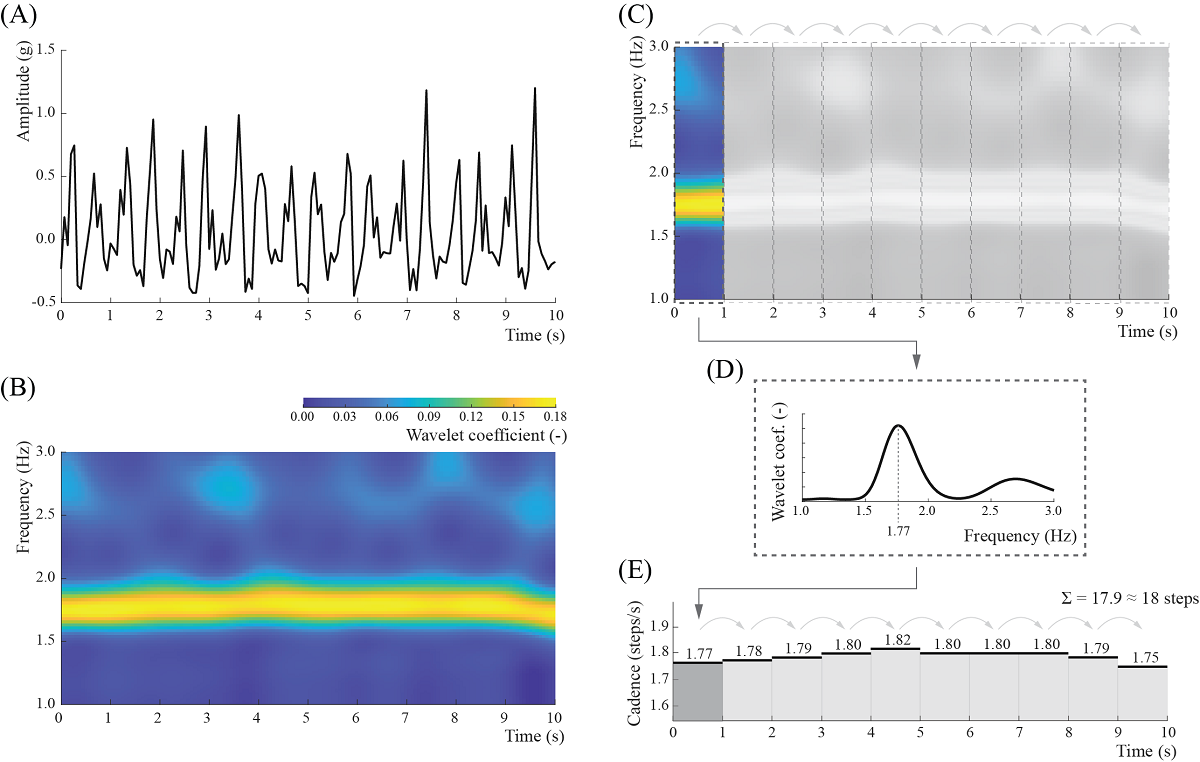
\includegraphics[width=.9\linewidth]{./images/straczkiewicz-wavelet-transform.png}
\caption{\label{fig:org155de56}(A) shows the accelerometer magnitude. (B) shows the accelerometer magnitude projected onto the time-frequency domain using wavelet transformation. Brighter colours represent frequencies that have higher weights or are more prominent in the signal. (C) is (B) split up into 1-second windows. (D) The step frequency is estimated to be the frequency with the highest average wavelet coefficient in each 1-second window. (E) The total number of steps is the sum of the steps in each 1-second window, rounded to the nearest integer. \cslcitation{18}{[18]}}
\end{figure}

The study made use of 7 publicly available data sets, as well as
its own additional study, totalling 255 participants.
The algorithm had excellent results for controlled situations,
with an error rate of less than 1\%, and was insensitive to
accelerometer positioning, which allows the algorithm to be
used on all kinds of accelerometer data to obtain a relatively
accurate step count.
However, the accuracy of the algorithm decreased when faced
with free living situations, as the steps were no longer consistent,
which inflated the overall step count.

\clearpage

Karas et al. \cslcitation{13}{[13]} made use of a concept similar to
continuous wavelet transformations to segment strides to count steps.
It makes use of a wavelet pattern that is estimated from the
given data and maximises the distance between the wavelet pattern,
translated and scaled, and the original signal (Figure \ref{fig:org2eefdab}).
The accelerometer data, which has been converted to a magnitude,
is first smoothed before the distance matrix is computed.
The result of the distance matrix computation is then tuned,
as the result only provides an initial estimate of
the stride location.
The computation produces an initial point and a scaling parameter
that corresponds to a specific length.
The result is then tuned by identifying the local maximum
of the smoothed accelerometer data within
two neighbourhoods centred around
the initial point and the initial point + specific length.

\begin{figure}[htbp]
\centering
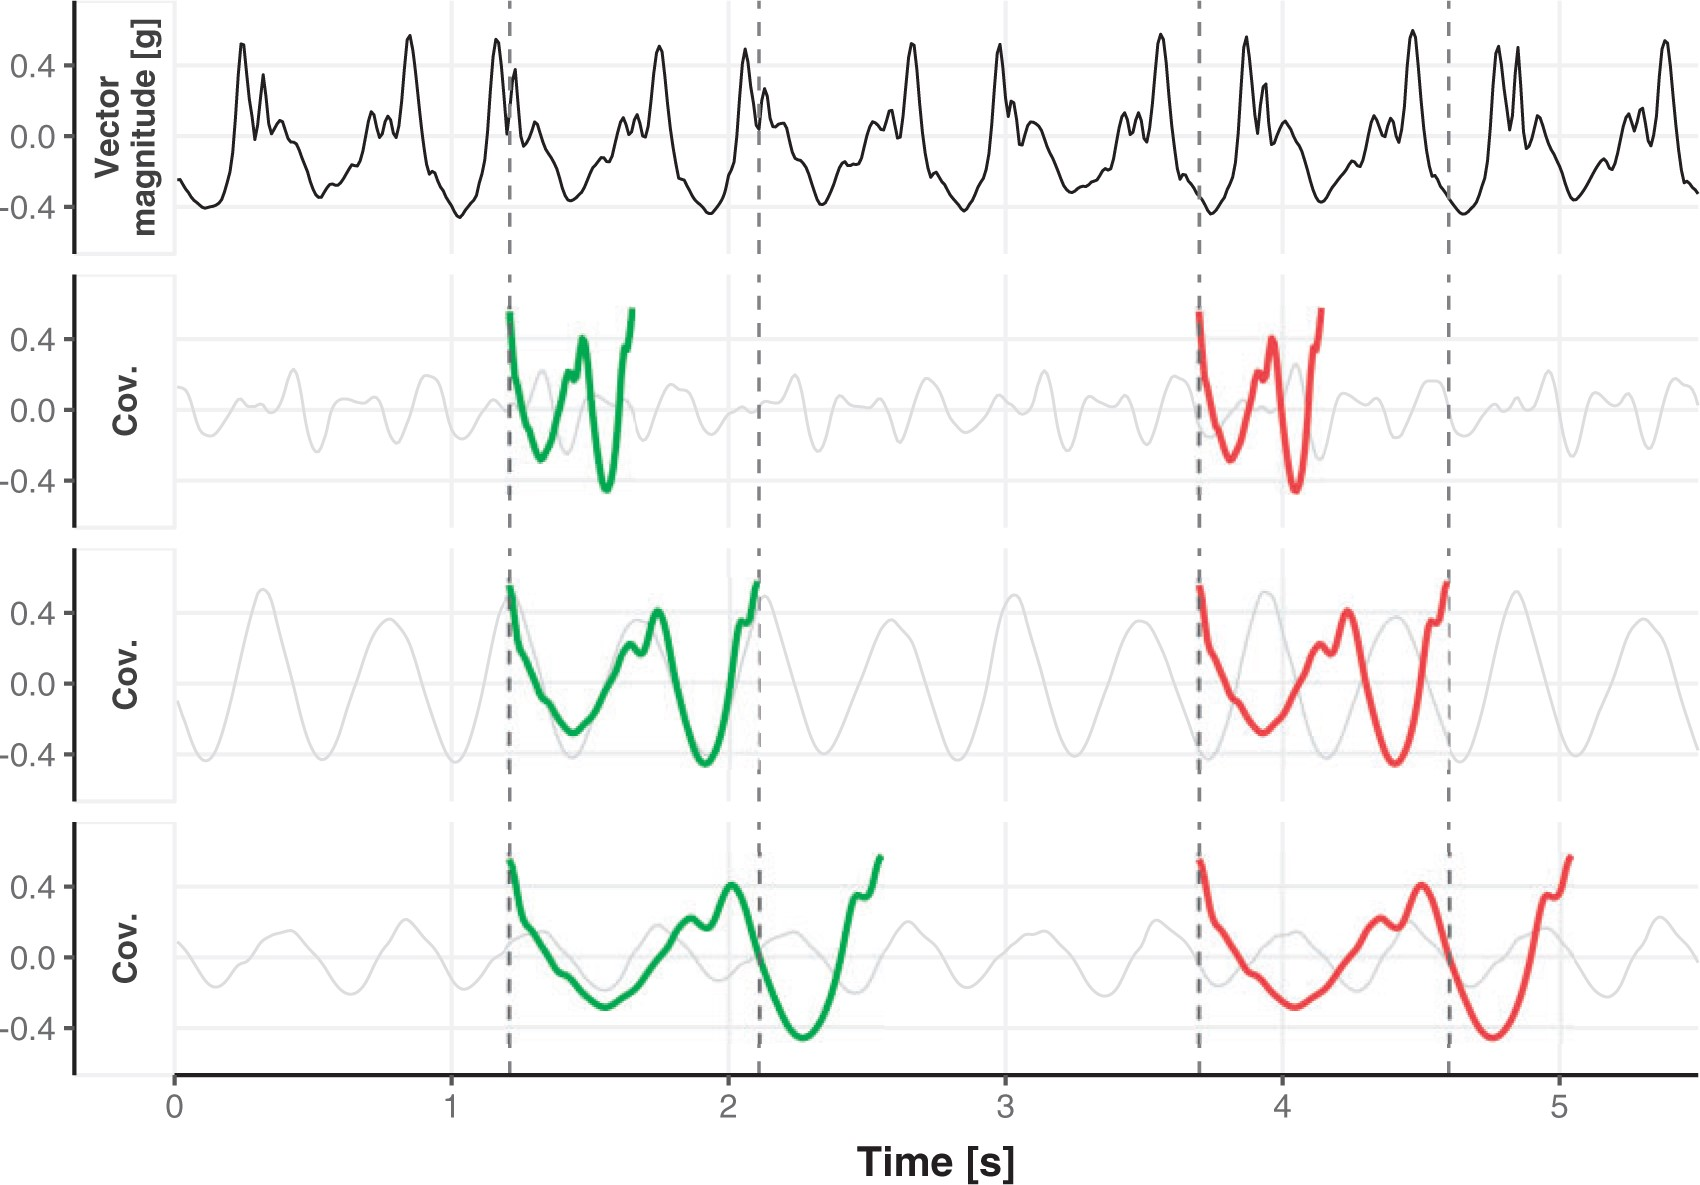
\includegraphics[width=.9\linewidth]{./images/adept-translation-and-scaling.jpeg}
\caption{\label{fig:org2eefdab}The first row shows the acceleration magnitude. The second to fourth rows show the covariance (muted grey lines in the background), and the wavelet pattern (red and green lines). \cslcitation{13}{[13]}}
\end{figure}

This segmentation of strides can then be used to effectively count
steps. The algorithm was found to be almost indistinguishable
from manual segmentation of strides for most accelerometer positions,
but had greater discrepancies for the non-dominant wrist,
with a per cent absolute deviation of 4.49\% for the left wrist,
0.75\% for the left hip, 0.95\% for the left ankle, and 0.85\%
for the right ankle.
The algorithm is also insensitive to the direction of the
accelerometer, which makes the algorithm more robust when
used in free-living conditions.

\clearpage

Finally, the most complex algorithm, by Small et al.
\cslcitation{15}{[15]} made use of a self-supervised
machine learning algorithm, making use of a ResNet-V2 neural network
with 18 layers and a 1-dimensional convolution layer with 10 million
parameters from a different study \cslcitation{19}{[19]}.
This neural network was trained to recognise human activity from
the massive UK Biobank accelerometer data set.
It had a relative improvement in the F1 score of 2.5\% to 130.9\%, with
a median of 24.4\% when compared to a random forest model trained
over the data set.

This machine learning algorithm was then trained
on the Oxwalk free living data set \cslcitation{21}{[21]}
to recognise gait patterns using PyTorch and Adam optimisation.
The predictions of this model on the training data set were
then used to train a Hidden Markov Model smoother, which was
then applied to the predictions in the test data set.
Afterwards, peak detection was done on the resulting windows that
were identified as walking using the \texttt{find\_peaks} function from
the SciPy Python package. The accelerometer data was first converted
into its magnitude, and gravity was subtracted from the data.
The acceleration data was then clipped for accelerations between
\(\pm \ 2 g\) and was passed through a 5 Hz low-pass filter before
being passed to the \texttt{find\_peaks} function.
The parameters to the \texttt{find\_peaks} function, specifically
minimum peak height, maximum peak width, and
minimum time between peaks, were iterated from 0.1 to \(1g\),
10 ms to 1 s and 0.2 to 2s, respectively.

The algorithm was found to have a mean absolute percentage error
of 12.5\%, a 1.3\% underestimation of steps and a correlation of
0.98 for the Oxwalk free-living data set.
The study also did external validation of other algorithms on
the same data set. Ducharme et al.'s \cslcitation{11}{[11]}
acceleration threshold algorithm resulted in a mean absolute
percentage error of 231.3\%, 69.1\% overestimation of steps, and
a correlation of 0.91. The Verisense algorithm
\cslcitation{12}{[12]} was better, but still produced
a mean absolute percentage error of 63.5\%, 7.2\% underestimation
of steps and a correlation of 0.85.
\section{Research gaps}
\label{sec:orgbf2f6f8}
Most of the reviewed papers have focused their attention on determining
step counts from just triaxial accelerometer data, making use of
increasingly complex algorithms to obtain more accurate readings based on
the acceleration magnitude. However, most smartphones, smartwatches
and fitness trackers have a gyroscope at least, and sometimes even
a magnetometer, making them 6-DOF or even 9-DOF IMUs. With a 6-DOF IMU,
one can make use of the extended Kalman filter
\cslcitation{22}{[22]}, \cslcitation{23}{[23]}, \cslcitation{24}{[24]}, or the more effective
Madgwick filter \cslcitation{25}{[25]}
to determine the orientation of the accelerometer.

These algorithms are highly efficient, with the Madgwick
filter outperforming the extended Kalman filter in efficiency,
and can be used in embedded systems.
These filters are often used in the aerospace industry to
determine the orientation of a drone or aircraft
and are used to automatically correct the craft's orientation.
The original implementation of the Madgwick filter is in C,
and was made to be run on embedded devices like IMUs and drones.

By making use of additional data, it would be possible to
simplify the algorithms needed to obtain an accurate step count,
reducing the need for machine learning algorithms which cannot be
run on embedded devices, and reduce the cost of analysing
accelerometer data, making step counting more accessible to more people.

However, most publicly available data sets for step counting do not
include gyroscope and magnetometer data, which means studies that
make use of 6-DOF or 9-DOF IMUs cannot make use of available data
to validate their algorithms, and must collect their own data sets.
This makes it far more difficult to develop a robust and accurate
algorithm that works well in free-living situations.

\clearpage

Moreover, all the studies reviewed in this paper, save for
Small et al.'s machine learning algorithm, which made use of the Oxwalk
data set containing data across different gait types, had a major caveat
to their results, which is the lack of representation of other gait types.
The studies mentioned that limping and other kinds of gait were
not considered in the development of their algorithms, and listed
it as a limitation of their study. While it is far easier to collect
accelerometer data with steps for normal and healthy participants,
physical activity tracking in healthcare is more concerned with
patients who have poor health, who are usually people with a disease,
or the elderly, both of whom usually have a different gait from
normal and healthy people. As such, different gait types should be
one of the first few considerations in such research,
especially when developing a step-counting algorithm for
healthcare physical activity tracking.

On a similar note, all the studies reviewed also did not look into
preventing participants from cheating the step counts by shaking the
device. This is expected since the studies looked at step counting
from a medical and personal activity tracking perspective,
and did not consider the commercial uses of step counting algorithms
in workplace step challenges. Other commercial uses of step
counting algorithms include cryptocurrency, with an example being
the \href{https://walken.io/}{Walken} token, which is earned by walking. Such commercial uses
of step counting place a large incentive for participants to cheat,
as these step challenges usually have rewards, and the cryptocurrency
has some real-world value, too. Hence, it is worthwhile to look into
a step-counting algorithm that can detect data that flouts the rules
of commercial step challenges and filter it out.

\clearpage

Furthermore, current and more recent research has
increasingly abstracted away the details in the accelerometer data,
by performing continuous wavelet
transformations to ignore the magnitude of acceleration and look
only to the oscillatory pattern of the data. Machine learning algorithms
take this further and obscure the method of determining what is and
isn't counted as a step, making the process a black box,
and unexplainable. This makes it far more difficult to modify
and build upon the algorithm.
While Small et al.'s \cslcitation{15}{[15]}
algorithm does not directly use machine learning algorithms to count
steps, the process of determining activity periods is still
obscured by the machine learning algorithm used.

Instead, more research should be done to understand the accelerometer
data, such as the correlations between certain movements and the
acceleration graph being plotted as a result. An increase in this
understanding would result in more efficient and simpler algorithms
that can be implemented in embedded devices, making step counting more
accessible to all.

These research gaps will be addressed in this study and
in the algorithm developed.
\chapter{Research methodology}
\label{sec:org3e3ac56}
\label{orga74852e}
In this study, preliminary data was first collected to gain a better
understanding of the accelerometer data and what it means.
Tiny sets of data, including just a single step,
with and without arm swing, and using different gaits, were
first plotted for analysis to have a better understanding of
how the body's movement is related to the acceleration data.
Afterwards, an algorithm was developed to catch all the edge
cases found in this preliminary data, and then further improved
after collecting the full data set.
\section{Overview of the step counting algorithm}
\label{sec:org5cce46e}
The main idea behind the algorithm is to make use of orientation
filters, such as the Madgwick orientation filter
\cslcitation{25}{[25]} to determine the orientation of
the accelerometer with respect to the global reference frame.
This is only possible with IMUs that are 6-DOF or 9-DOF,
providing triaxial gyroscope and optionally magnetometer data.
With this information, it is now possible to resolve the
triaxial acceleration in the local reference frame of the
accelerometer into the global reference frame.
The resolved acceleration vectors in the x-direction, y-direction
and z-direction represent the vectors in the forward-backwards direction,
left-right direction, and up-down direction, respectively.

For step counting, the acceleration in the forward-backwards and left-right
directions are not particularly useful, especially for an accelerometer
that is wrist-mounted, as it is subject to a lot of noise.
Hence, instead of performing analysis on the acceleration
magnitude, analysis is performed on only the up-down acceleration vector,
as the peaks and troughs in the up-down direction are indicative of
the steps taken by a person, while the acceleration vectors in the
front-back direction and left-right direction are mostly noise.
However, this noise in the front-back and the left-right directions
should not be immediately discarded, as there is a possibility
of them providing useful information.

\clearpage

The algorithm is as follows:
\begin{enumerate}
\item Make a copy of the raw data.
\item Apply a 4th-order Butterworth low-pass filter of 3 Hz
to remove high-frequency noise in the accelerometer data.
The gyroscope and magnetometer data are not filtered.
\item Apply the Madgwick orientation filter on the data to obtain
the corresponding IMU orientations in the global reference frame.
\item Obtain a direction cosine matrix for each of the IMU orientations,
which is a rotation matrix that, when multiplied by the cardinal
direction vectors (1, 0, 0), (0, 1, 0), (0, 0, 1), will return
the basis vectors representing the orientation of the IMU.
\item Take the negative of the direction cosine matrix found in the
previous step, and multiply it by the corresponding
acceleration vector. This is a change-of-basis operation to
convert the acceleration vectors in the accelerometer's local
reference frame to the global reference frame.
\item Take the dot product of the acceleration vectors found in the previous
step and each of the cardinal direction vectors
(1, 0, 0), (0, 1, 0), (0, 0, 1) and sum up the result
to obtain the projection of the acceleration vectors
in the cardinal directions. This will return the vectors
representing the accelerations in the cardinal directions.
\item Perform peak or trough finding on the z-direction or
up-down acceleration vector to obtain a tentative step count.
\item Filter the tentative step count based on additional heuristics
and thresholds, such as making use of a minimum acceleration
threshold to reject noise, limiting the number of possible orientations
in a window to a certain number, analysing the raw data to find
absurd acceleration values that can only mean the data is cheated, etc.
\end{enumerate}

\clearpage

Below is a flow chart of the algorithm:
% Start and stop box
\tikzstyle{startstop} = [
    rectangle,
    rounded corners,
    minimum width=3cm,
    minimum height=1cm,
    text centered,
    draw=black,
    fill=red!30
]

% Input and output box
\tikzstyle{io} = [
    trapezium,
    trapezium left angle=70,
    trapezium right angle=110,
    minimum width=3cm,
    minimum height=1cm,
    text width=3.5cm,
    text centered,
    draw=black,
    fill=blue!30
]

% Process blocks
\tikzstyle{process} = [
    rectangle,
    minimum width=3cm,
    minimum height=1cm,
    text centered,
    text width=4cm,
    draw=black,
    fill=orange!30
]

% Decision block
\tikzstyle{decision} = [
    diamond,
    minimum width=3cm,
    minimum height=1cm,
    text centered,
    draw=black,
    fill=green!30
]

% Arrow style
\tikzstyle{arrow} = [thick,->,>=stealth]

% The actual flowchart
\begin{center}
\begin{tikzpicture}[node distance=1cm]

% Start of the algorithm
\node (start) [startstop] {Start};

% Accelerometer data input
\node (gyroscope) [io, below=of start] {Triaxial gyroscope data};
\node (magnetometer) [io, right=of gyroscope] {Triaxial magnetometer data (optional)};
\node (accelerometer) [io, left=of gyroscope] {Triaxial accelerometer data};

% 4th order Butterworth filter
\node (lowpass) [process, below=of accelerometer] {4th order Butterworth low-pass filter};

% Madgwick orientation filter
\node (madgwick) [process, right=of lowpass] {Madgwick orientation filter};

% Get direction cosine matrix
\node (dcm) [process, right=of madgwick] {Obtain direction cosine matrix};

% Change of basis
\node (changebasis) [process, below=of dcm] {Change acceleration vector basis to the basis of the global reference frame};

% Obtain projections
\node (projection) [process, left=of changebasis] {Obtain projection of the vectors in the cardinal directions};

% Perform peak or trough finding
\node (findpeaks) [process, left=of projection] {Find peaks or troughs};

% Filter the step count
\node (stepfilter) [process, below=of findpeaks, yshift=-0.5cm] {Filter for valid step counts};

% Output step count
\node (output) [io, right=of stepfilter, text width=2.5cm, xshift=0.5cm] {Final step count};

% Stop node
\node (stop) [startstop, right=of output, xshift=1.25cm] {Stop};

% Arrows
\draw [arrow] (start) -- (accelerometer);
\draw [arrow] (start) -- (gyroscope);
\draw [arrow] (start) -- (magnetometer);
\draw [arrow] (accelerometer) -- (lowpass);
\draw [arrow] (lowpass) -- (madgwick);
\draw [arrow] (gyroscope) -- (madgwick);
\draw [arrow] (magnetometer) -- (madgwick);
\draw [arrow] (madgwick) -- (dcm);
\draw [arrow] (dcm) -- (changebasis);
\draw [arrow] (changebasis) -- (projection);
\draw [arrow] (projection) -- (findpeaks);
\draw [arrow] (findpeaks) -- (stepfilter);
\draw [arrow] (stepfilter) -- (output);
\draw [arrow] (output) -- (stop);

\end{tikzpicture}
\end{center}

\clearpage

For exact implementation details regarding the algorithm,
please refer to the \hyperref[orgf85d410]{appendix}.
Alternatively, you can view the implementation in the
\texttt{algorithm.py} file distributed together with this paper.

Currently, only a Python implementation
making use of the libraries \href{https://numpy.org/}{NumPy}, \href{https://pandas.pydata.org/}{Pandas}, \href{https://scipy.org/}{SciPy}, \href{https://matplotlib.org/}{Matplotlib},
and \href{https://ahrs.readthedocs.io/en/latest/}{AHRS} is available.
A C implementation for this algorithm would be ideal,
as one of the objectives of this research is to have the algorithm run
on embedded devices.

The algorithm is open-source and is released under an open-source
licence that allows anyone to reuse, distribute and modify,
as this is the main goal for the development of this algorithm.

\clearpage
\section{Data collection}
\label{sec:org303f7f9}
\label{orgdcbbb87}
Accelerometer data was self-collected
using a \href{https://witmotion-sensor.com/collections/bluetooth-accerometer/products/bluetooth-5-0-accelerometer-inclinometer-wt901blecl-mpu9250-high-precision-9-axis-gyroscope-anglexy-0-05-accuracy-magnetometer-with-kalman-filter-low-power-3-axis-ahrs-imu-sensor-for-arduino}{WitMotion WT901BLECL 9-DOF IMU},
as publicly available data sets do not contain gyroscope
or magnetometer data.
The accelerometer data has a sampling frequency of 100 Hz.
The accelerometer makes use of Bluetooth 5.0 and a mobile application
to stream data to the phone, where it is subsequently saved
in a tab-separated values (TSV) file with a \texttt{.txt} extension.

\begin{figure}[h]
    \centering
    \begin{subfigure}[b]{0.24\textwidth}
        \centering
        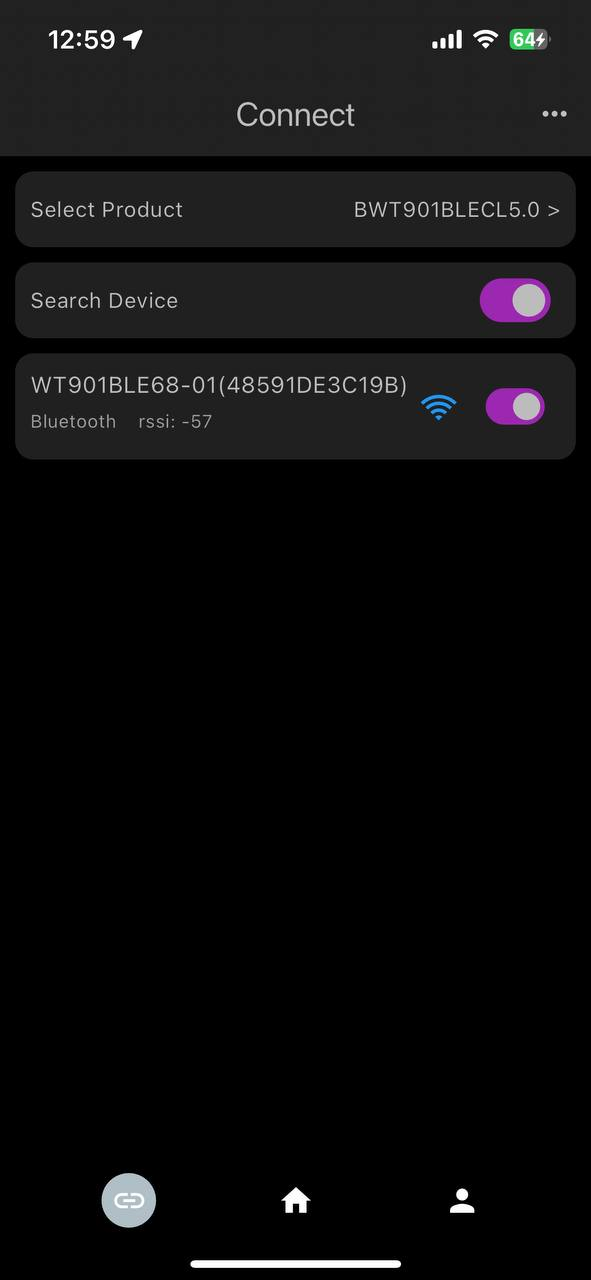
\includegraphics[width=\textwidth]{witmotion-app-interface-connect-screen}
    \end{subfigure}
    \begin{subfigure}[b]{0.24\textwidth}
        \centering
        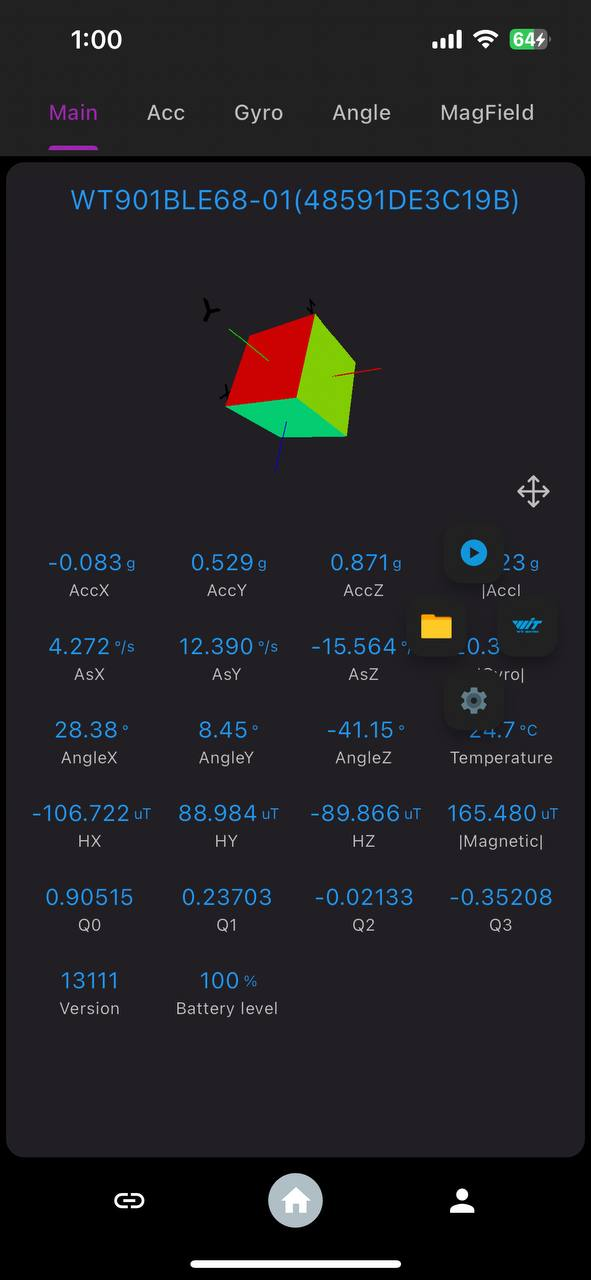
\includegraphics[width=\textwidth]{witmotion-app-interface-accelerometer-overview-screen}
    \end{subfigure}
    \begin{subfigure}[b]{0.24\textwidth}
        \centering
        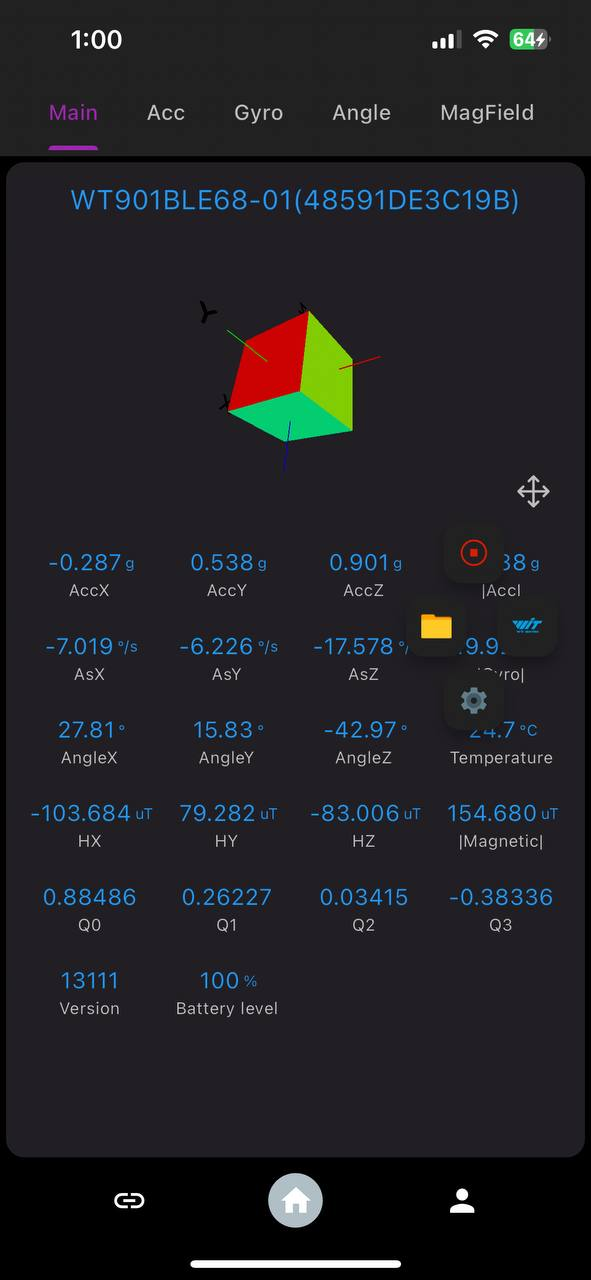
\includegraphics[width=\textwidth]{witmotion-app-interface-accelerometer-recording-screen}
    \end{subfigure}
    \begin{subfigure}[b]{0.24\textwidth}
        \centering
        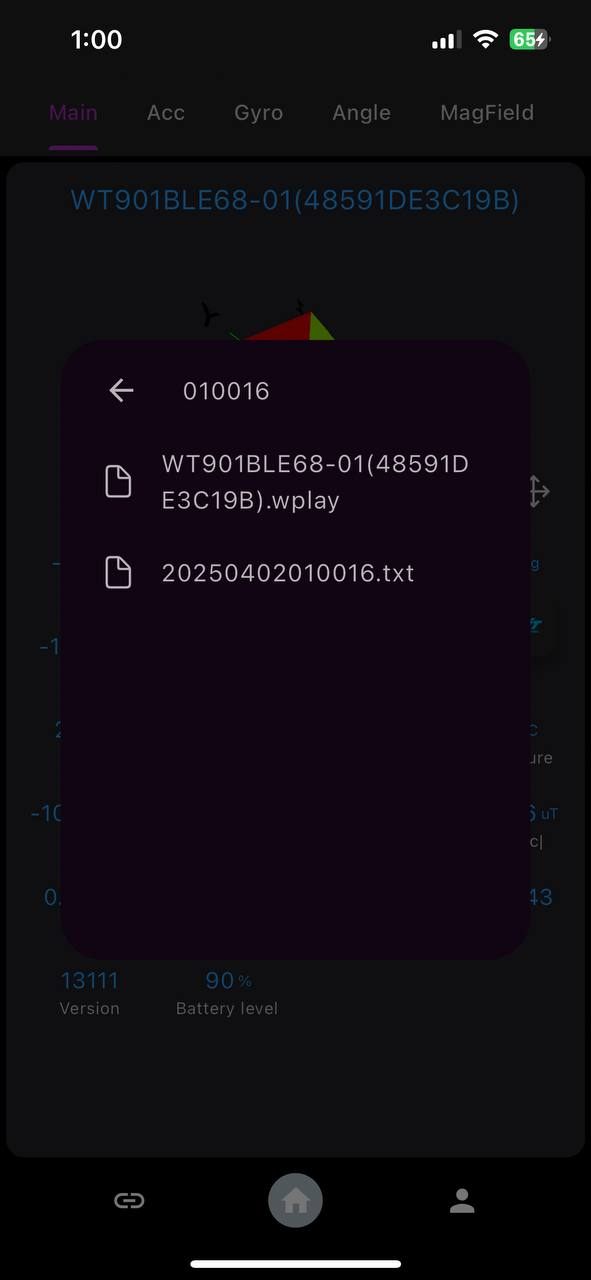
\includegraphics[width=\textwidth]{witmotion-app-interface-accelerometer-data-screen}
    \end{subfigure}
    \caption{The WitMotion application interface.}
\end{figure}

\clearpage

The accelerometer is mounted snugly on the dominant wrist
(right wrist) using a ribbon that is tied around the accelerometer
to loop around the wrist to ensure a snug fit.
The accelerometer still has some movement, but it is not excessive.

\begin{figure}[htbp]
\centering
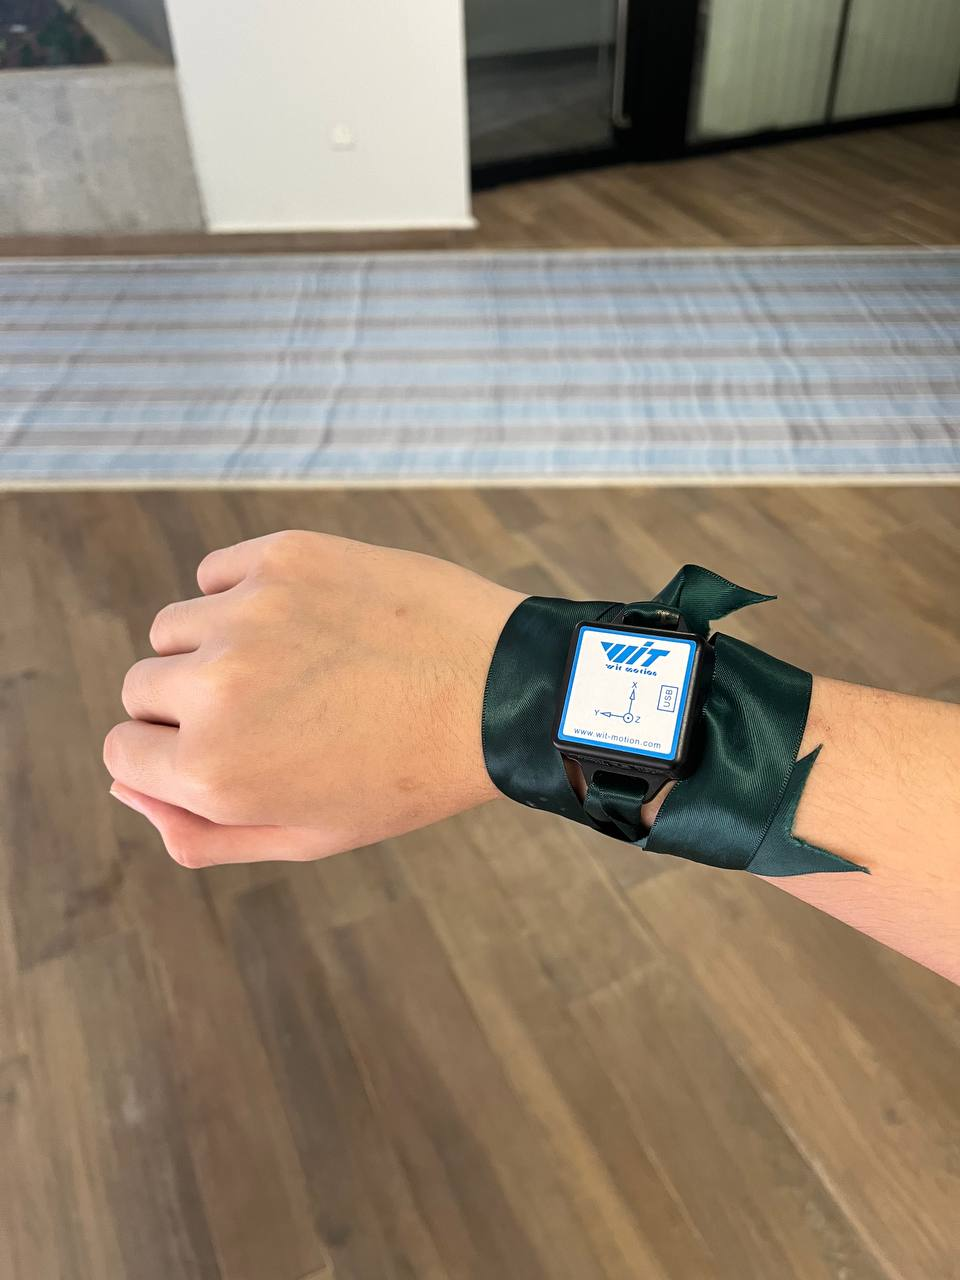
\includegraphics[height=20em]{./images/accelerometer-mounting.jpg}
\caption{The mounting of the WitMotion accelerometer.}
\end{figure}

\clearpage

The number of steps for the ground truth is obtained by
manually counting a predetermined number of steps,
usually 50 steps.
The data collected includes 10 sets of 50 steps for walking, running,
and shuffling, all of which have arm swing,
as well as 50 sets of 12 steps for both climbing up and down stairs,
and 100 steps for limping.
The data set for climbing up stairs has arm swing,
while the data set for climbing down stairs has no arm swing.
For limping, two steps are counted when the limping individual
places their front foot on the ground, and drags their back leg
forward to join their front leg.

The location where the data is collected is floor B2
of Nanyang Technological University's Academic Building North,
which is a flat area with no slopes.

\begin{figure}[h]
    \centering
    \begin{subfigure}[b]{0.19\textwidth}
        \centering
        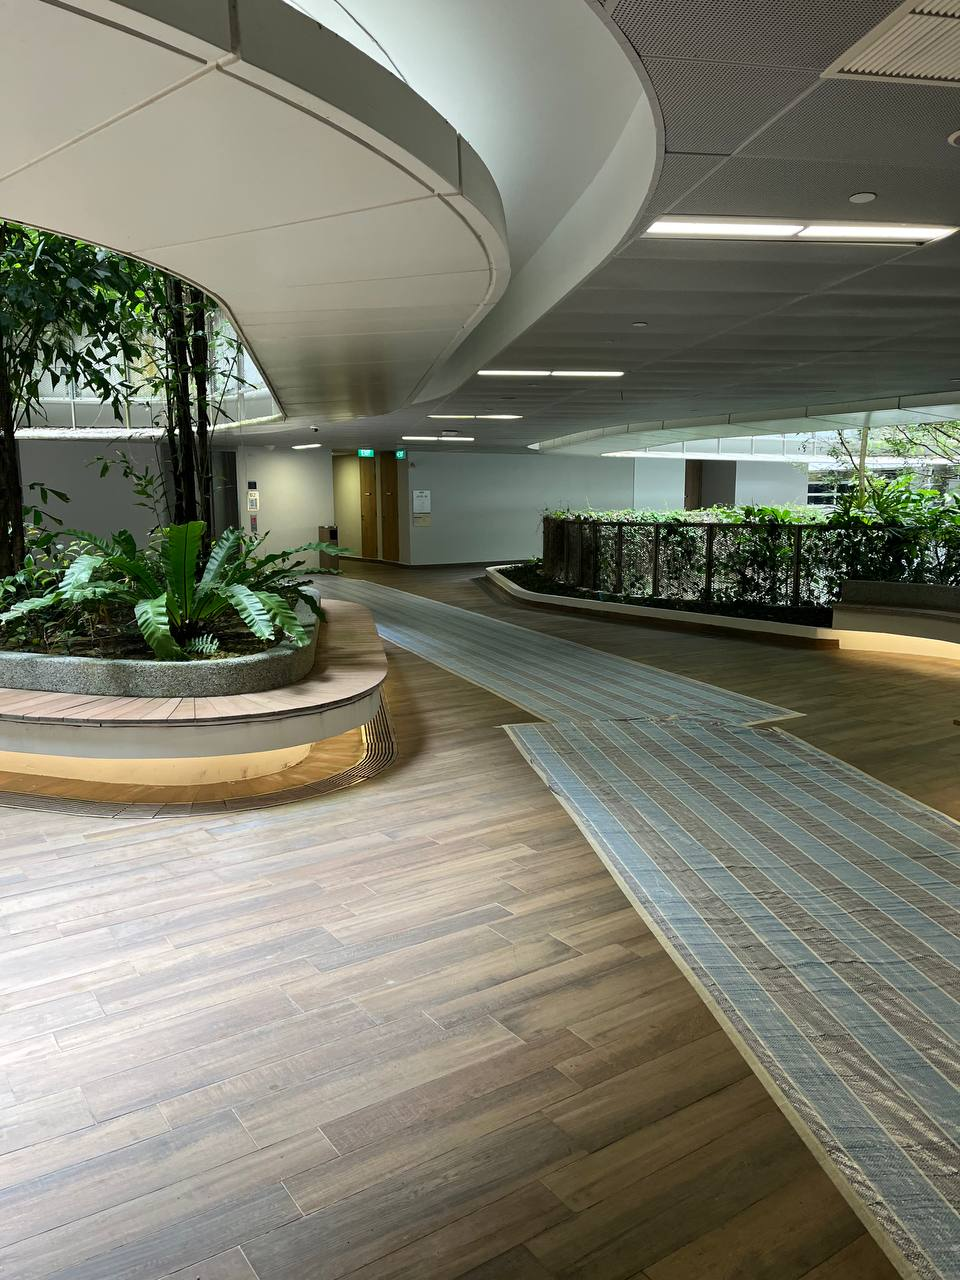
\includegraphics[width=\textwidth]{walking-area-1}
    \end{subfigure}
    \begin{subfigure}[b]{0.19\textwidth}
        \centering
        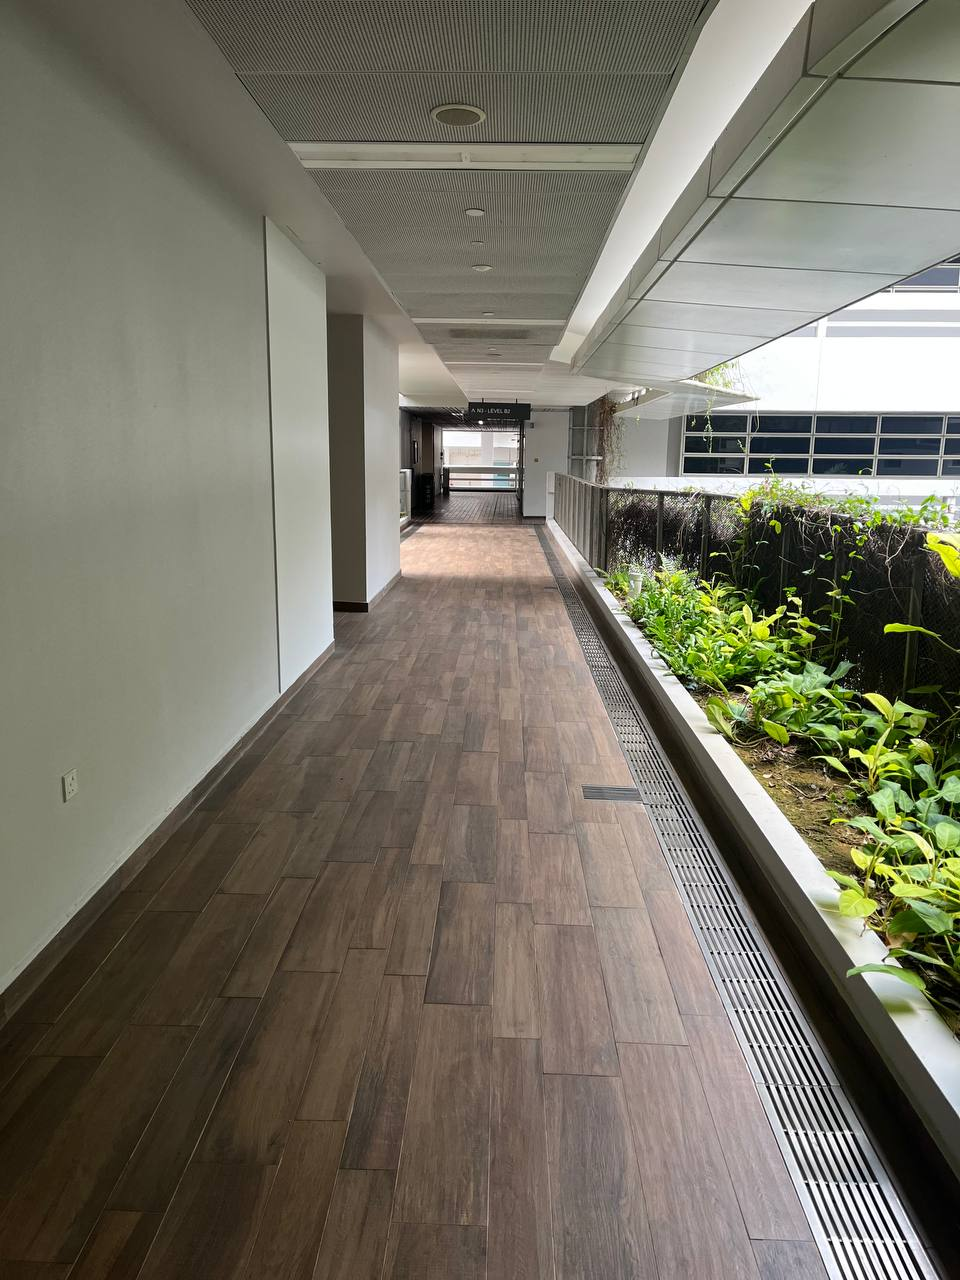
\includegraphics[width=\textwidth]{walking-area-2}
    \end{subfigure}
    \begin{subfigure}[b]{0.19\textwidth}
        \centering
        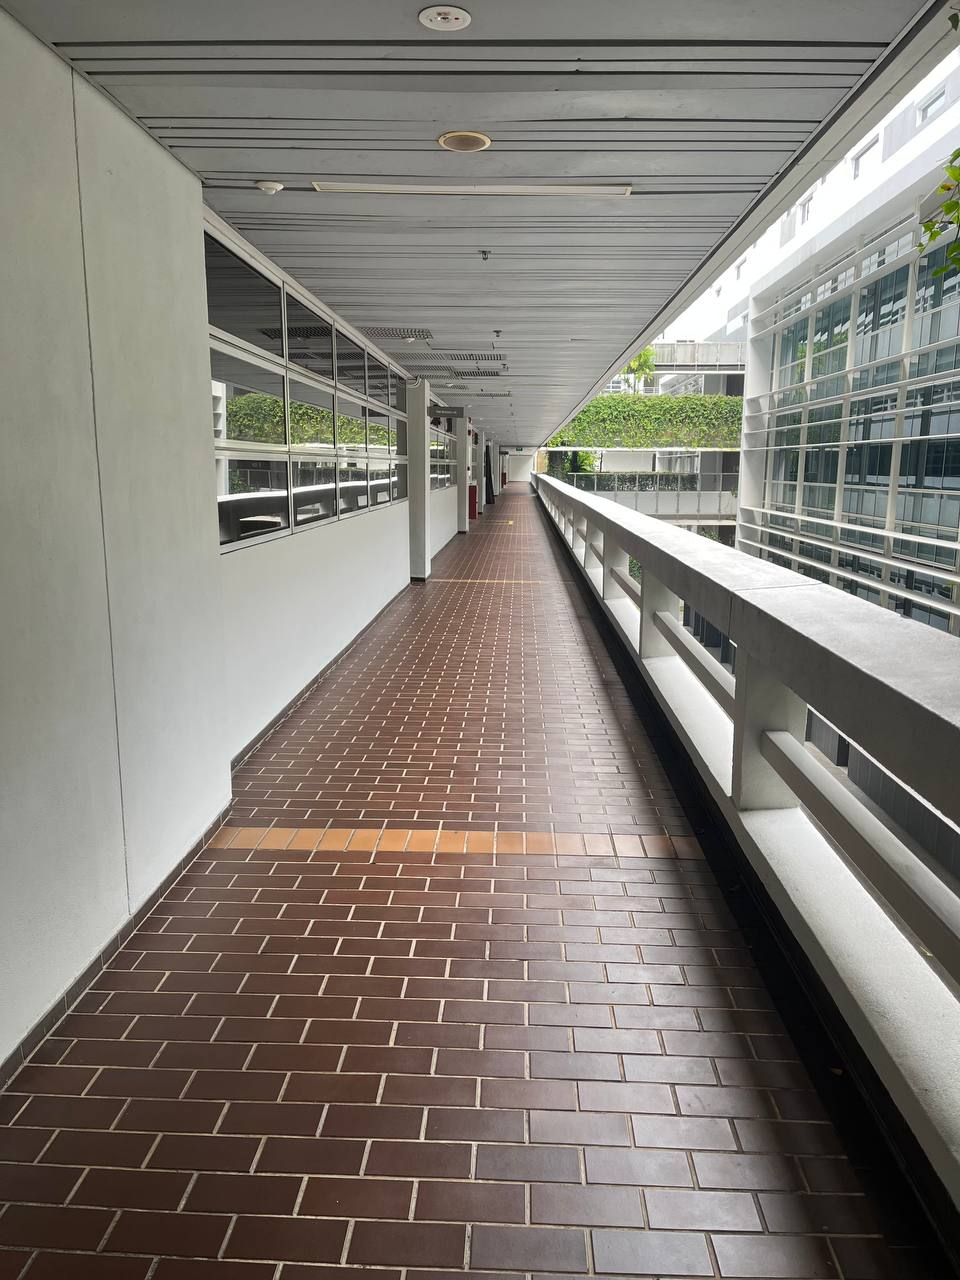
\includegraphics[width=\textwidth]{walking-area-3}
    \end{subfigure}
    \begin{subfigure}[b]{0.19\textwidth}
        \centering
        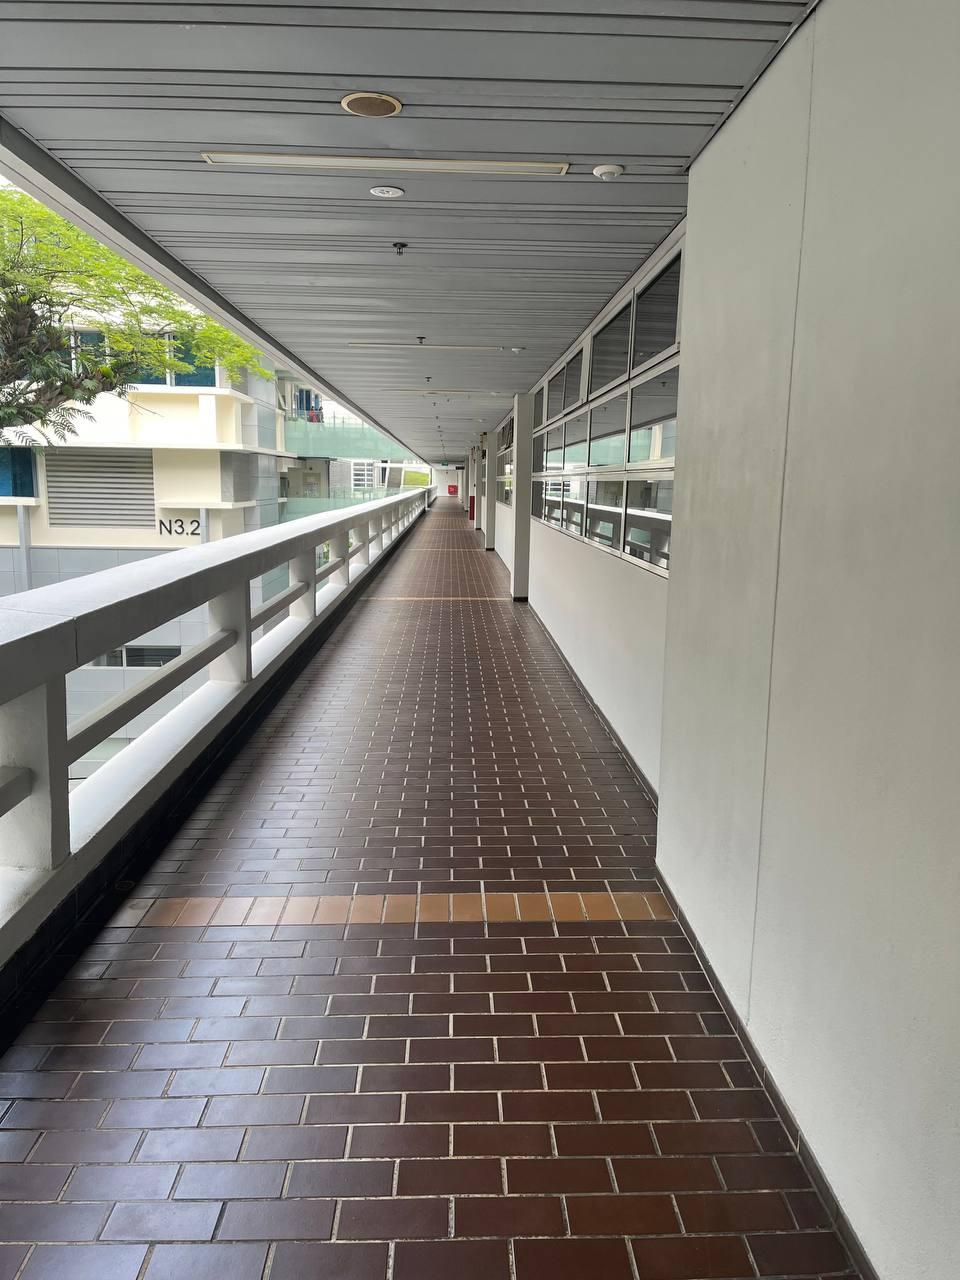
\includegraphics[width=\textwidth]{walking-area-4}
    \end{subfigure}
    \begin{subfigure}[b]{0.19\textwidth}
        \centering
        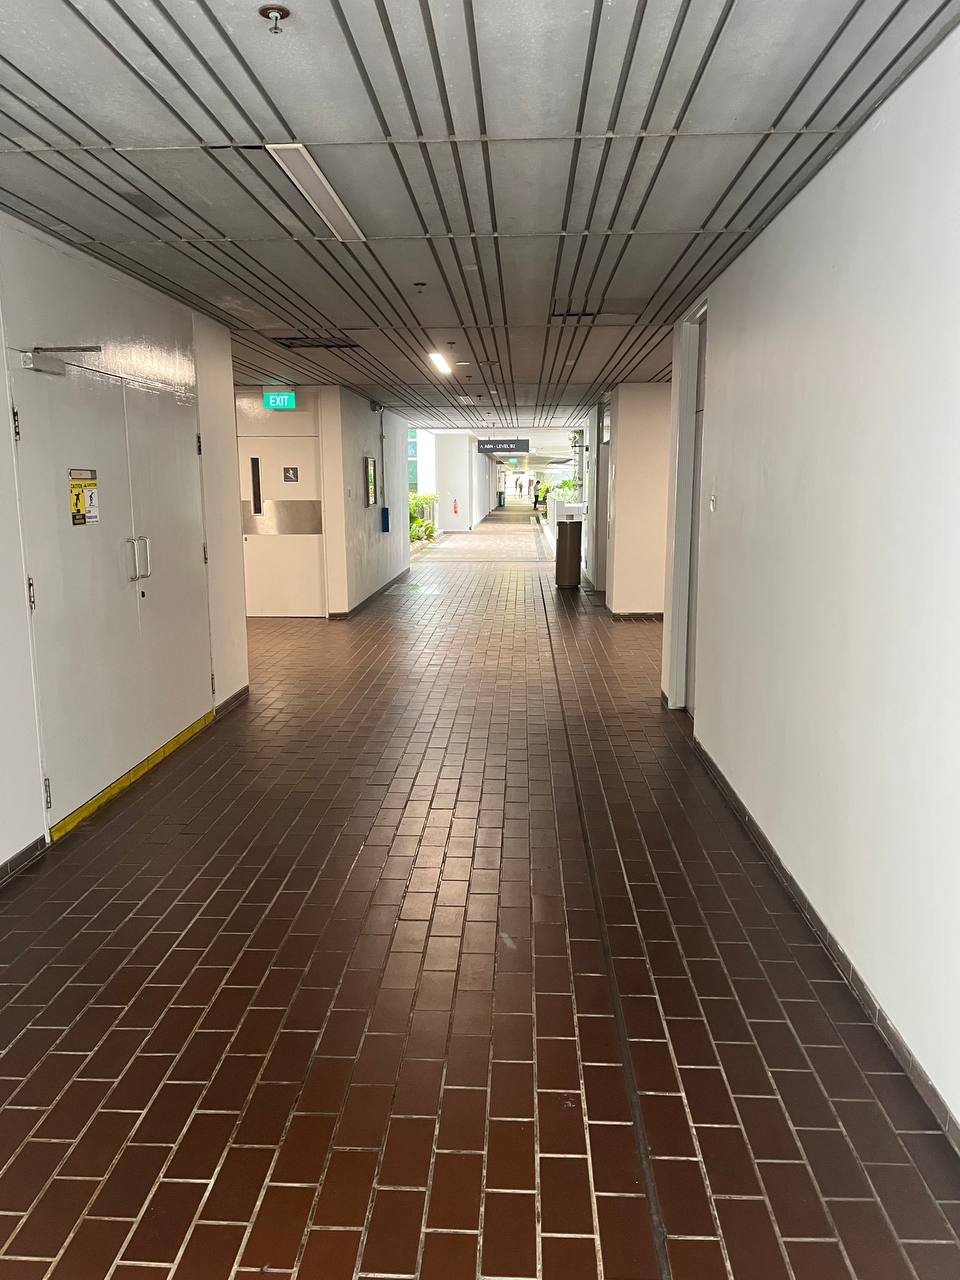
\includegraphics[width=\textwidth]{walking-area-5}
    \end{subfigure}
    \caption{Images of the location where data is collected.}
\end{figure}

\begin{figure}[h]
    \centering
    \begin{subfigure}[b]{0.26\textwidth}
        \centering
        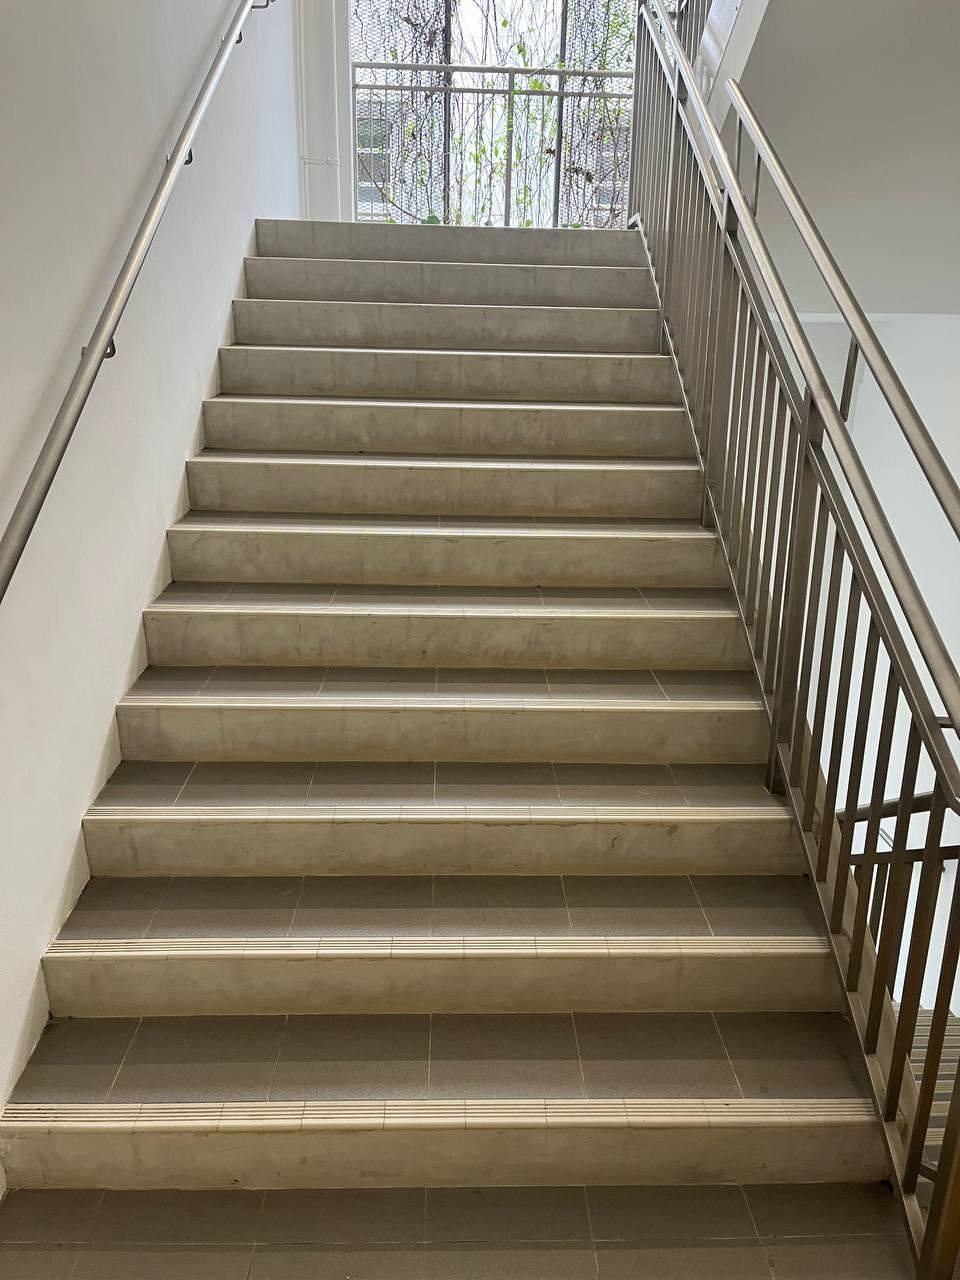
\includegraphics[width=\textwidth]{stairs-up}
    \end{subfigure}
    \begin{subfigure}[b]{0.26\textwidth}
        \centering
        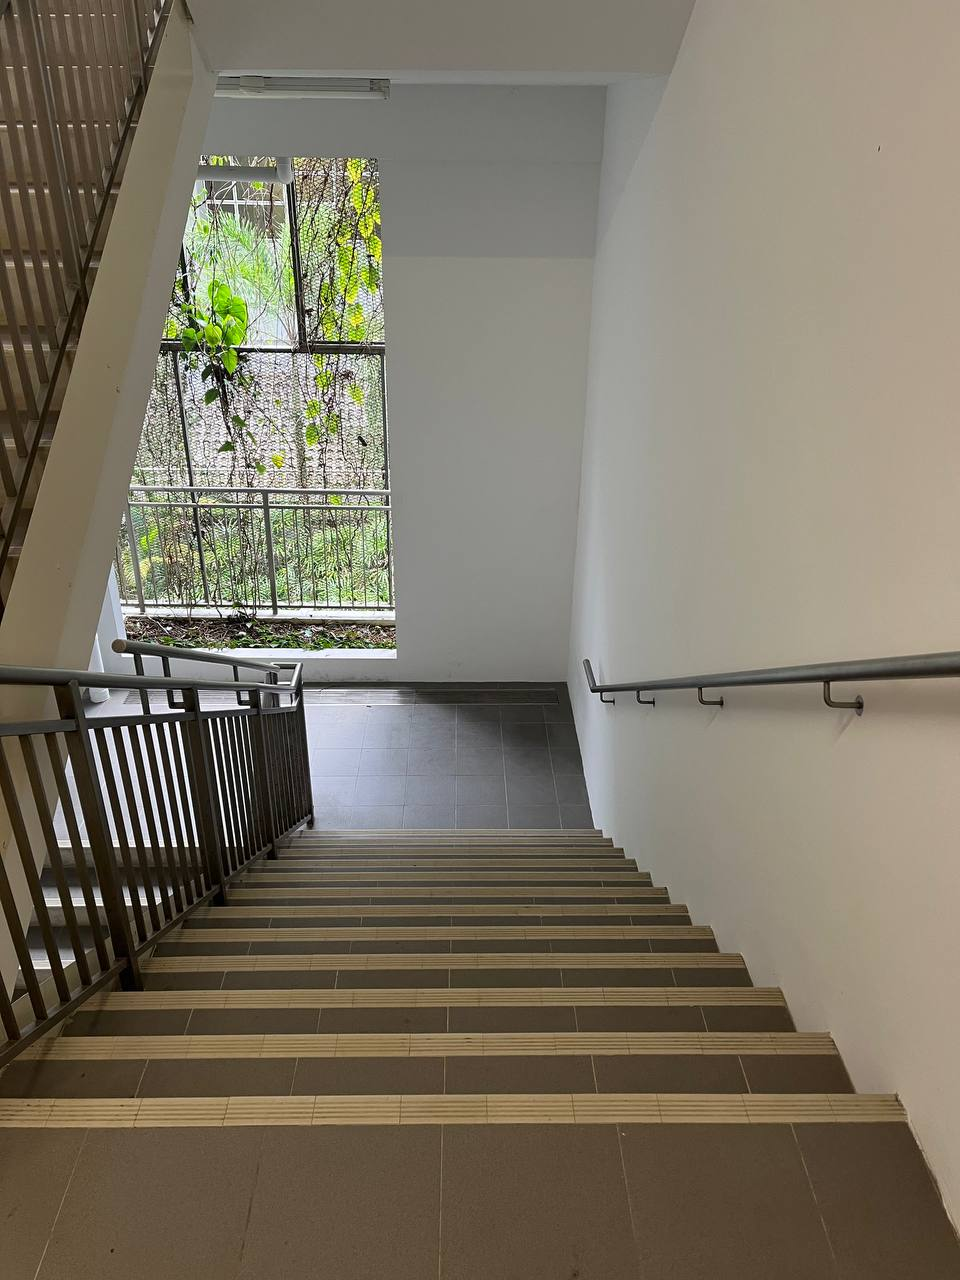
\includegraphics[width=\textwidth]{stairs-down}
    \end{subfigure}
    \caption{Images of the stairs where data is collected.}
\end{figure}
\chapter{Results and discussion}
\label{sec:org46cd857}
\label{orgb796370}
\section{Walking}
\label{sec:orgc0160a3}

\subsection{50 steps data set}
\label{sec:orged2f1e5}
The details of how the data for the 50 steps data set is
collected is detailed in the \hyperref[orgdcbbb87]{data collection} section.
\phantomsection
\label{org5d2a2b2}
\begin{verbatim}
Below are the accuracy metrics:

Maximum error: 3
Mean absolute percentage error: 0.013999999999999999
Mean squared error: 1.3
Root mean squared error: 1.140175425099138
\end{verbatim}

\begin{center}
\includegraphics[width=.9\linewidth]{./.ob-jupyter/7c9961b2a1e1155c5d750ef242d693b70b2154f2.png}
\end{center}

As seen from the box plot and the accuracy metrics above,
the algorithm performs quite well for counting walked steps.
\subsection{500 steps data set}
\label{sec:org3ff3efc}
The 500-step data set is collected in the same way as the 50-step
data set, but the ground truth value varies a little due to the
difficulty in ensuring that the walking person stops walking
after walking exactly 500 steps.
\phantomsection
\label{org923d629}
\begin{verbatim}
Below are the accuracy metrics:

Maximum error: 201
Mean absolute percentage error: 0.2988
Mean squared error: 23379.0
Root mean squared error: 152.90192935342574
\end{verbatim}

\begin{center}
\includegraphics[width=.9\linewidth]{./.ob-jupyter/a65bd80dc938c34a8bbdf1d8842e78571db3fcf7.png}
\end{center}

From the box plot and the accuracy metrics above, the algorithm's
accuracy decreased quite significantly when counting a larger
number of steps at a time. This is mostly due to the stepping
speed varying throughout, with higher stepping speed causing the
step counting algorithm to miss steps,
resulting in undercounted steps.
\section{Running}
\label{sec:org6134095}
The running data set is collected as detailed in the
\hyperref[orgdcbbb87]{data collection section}.
\phantomsection
\label{org84c5160}
\begin{verbatim}
Below are the accuracy metrics:

Maximum error: 2
Mean absolute percentage error: 0.025490196078431372
Mean squared error: 2.1
Root mean squared error: 1.449137674618944
\end{verbatim}

\begin{center}
\includegraphics[width=.9\linewidth]{./.ob-jupyter/4047eb122907d6a2bf6fa79ba3c707b57905d2f7.png}
\end{center}

As seen from the box plots and accuracy metrics above,
the algorithm is quite accurate for running.
\section{Limping}
\label{sec:org26fb283}
The limping data set is collected as detailed in the
\hyperref[orgdcbbb87]{data collection section}.
\phantomsection
\label{org91b3808}
\begin{verbatim}
Below are the accuracy metrics:

Maximum error: 2
Mean absolute percentage error: 0.009999999999999998
Mean squared error: 1.4
Root mean squared error: 1.1832159566199232
\end{verbatim}

\begin{center}
\includegraphics[width=.9\linewidth]{./.ob-jupyter/1a90a911ff11f251f52a87c4c1e12615295a3468.png}
\end{center}

\clearpage

As seen from the box plots and accuracy metrics above,
the algorithm is quite accurate for limping,
even exceeding the algorithm's accuracy for walking and running.
This is a surprising result,
as it was initially expected that the algorithm would not pick up
on the step counts from the back leg being dragged forward.

This suggests that when limping, the person lifts their body up
significantly to reduce the acceleration before dragging their back
foot forward, which would cause the acceleration to spike before
dipping back down to the value of gravity, which would be considered
a trough by the algorithm, and hence sufficient to count as a step.
\section{Shuffling}
\label{sec:org07aefe9}
The shuffling data set is collected as detailed in the
\hyperref[orgdcbbb87]{data collection section}.
\phantomsection
\label{org366d03b}
\begin{verbatim}
Below are the accuracy metrics:

Maximum error: 18
Mean absolute percentage error: 0.154
Mean squared error: 91.3
Root mean squared error: 9.555103348473002
\end{verbatim}

\begin{center}
\includegraphics[width=.9\linewidth]{./.ob-jupyter/45535756695996a7fedf1b9dacf67909b3de48f4.png}
\end{center}

\clearpage

As seen from the box plot and the accuracy metrics above,
the algorithm performs expectedly poorly for counting steps that are
not well-defined, as is often the case for shuffling.
The algorithm relies on finding peaks that are of a sufficient height
to count a step, and since shuffling usually results in
small changes in acceleration as the foot is not lifted,
shuffled steps are not picked up by the algorithm.
\section{Climbing stairs}
\label{sec:org9190638}

\subsection{Climbing up stairs}
\label{sec:org604e945}
The data set for climbing up stairs is collected as detailed in the
\hyperref[orgdcbbb87]{data collection section}.
\phantomsection
\label{org55268b9}
\begin{verbatim}
Below are the accuracy metrics:

Maximum error: 5
Mean absolute percentage error: 0.10333333333333333
Mean squared error: 2.92
Root mean squared error: 1.7088007490635062
\end{verbatim}

\begin{center}
\includegraphics[width=.9\linewidth]{./.ob-jupyter/46796909e5fb51097821f529d305efcc3b545e7e.png}
\end{center}

As seen from the box plot and the accuracy metrics above,
algorithm performs poorly for counting steps when climbing up stairs,
and misses a lot of steps.
\subsection{Climbing down stairs}
\label{sec:orgac4700a}
The data set for climbing down stairs is collected as detailed in the
\hyperref[orgdcbbb87]{data collection section}.
\phantomsection
\label{orgea19e25}
\begin{verbatim}
Below are the accuracy metrics:

Maximum error: 6
Mean absolute percentage error: 0.2316666666666667
Mean squared error: 9.62
Root mean squared error: 3.1016124838541645
\end{verbatim}

\begin{center}
\includegraphics[width=.9\linewidth]{./.ob-jupyter/225a7683d3918b119f34380d42d665a028becd8c.png}
\end{center}

As seen from the box plot and the accuracy metrics above,
algorithm also performs poorly for counting steps when
climbing down stairs, and misses a lot of steps.
\subsection{Explanation}
\label{sec:orgd49675c}
The cause of undercounting steps in the algorithm
when climbing stairs is likely due to uneven steps.

For individuals who climb stairs unevenly, meaning the second step
is taken much faster than the first step, the accelerometer would not
be able to pick up on the change in acceleration, as the acceleration
spike due to lifting the second foot is almost fully neutralised
by the acceleration drop due to the placement of the first foot.

This results in the algorithm missing steps due to the acceleration
not passing the threshold to be counted as a step. Such uneven steps
also make it difficult for algorithms based on accelerometer data to
pick up on a step, as the acceleration is neutralised and will look
like just one step. A heuristic will likely be needed to detect such
an occurrence of uneven steps and compensate for the missing steps.

On the other hand, for individuals who are very even in their steps,
meaning their first step and second step take a similar
amount of time, would allow the algorithm to pick up on the
steps taken, as the spike in acceleration from the lifting of the
second foot is not being neutralised by the placement of the
first foot.

This result is likely generalisable to counting steps in general,
as this problem is also the likely explanation for the significant
undercounting of steps in the larger 500-step walking data set,
which had a higher stepping frequency than the 50-step data set.
\section{Miscellaneous}
\label{sec:org255c409}

\subsection{Manual shaking}
\label{sec:orgd0ed701}
The manual shaking data set is data from manually shaking the
accelerometer for a few seconds. The data set considers the
different ways to shake the accelerometer, such as shaking it
in the up-down, left-right, and forward-backward directions.
Twirling the accelerometer in a circular motion is also considered.

This set of data is only collected once, and it is used to develop
the heuristic for excluding steps that are most likely due to
shaking. Ideally, more data should be collected for the manual
shaking of the accelerometer, but the algorithm is
sufficiently generalisable as it detects peaks of more than
\(\qty{100}{m.s^{-2}}\) in the 5 to 7 Hz frequency range,
which is characteristic of manually shaking the accelerometer.

\clearpage

\phantomsection
\label{org7c7cff1}
\begin{verbatim}
Below are the accuracy metrics:

Maximum error: 0
Mean absolute percentage error: 0.0
Mean squared error: 0.0
Root mean squared error: 0.0
\end{verbatim}

\begin{center}
\includegraphics[width=.9\linewidth]{./.ob-jupyter/a6867ed972c0b3e52cba04a2b616d989186c0db4.png}
\end{center}

As seen from the box plot and accuracy metrics above,
the algorithm successfully filters out cheated accelerometer data
through shaking the accelerometer,
while remaining fairly accurate for legitimate data.
\subsection{Eating pasta}
\label{sec:orga603050}
The eating pasta data set was also only collected once, and it is an
initial attempt in making the algorithm more accurate in free living
situations where there is a lot of hand movement that is not due to
walking or running.
\phantomsection
\label{org6ad30e2}
\begin{verbatim}
Below are the accuracy metrics:

Maximum error: 6
Mean absolute percentage error: 2.7021597764222976e+16
Mean squared error: 36.0
Root mean squared error: 6.0
\end{verbatim}

\begin{center}
\includegraphics[width=.9\linewidth]{./.ob-jupyter/d43f434960abccdc14fc8245464562b8c035ced6.png}
\end{center}

As seen from the box plot and the accuracy metrics above,
the algorithm handles a free-living situation like eating pasta
with decent accuracy, but far more data should be collected
to test the effectiveness of the algorithm in other
free living situations, as this piece of data only accounts for
one free living situation, which is eating pasta.
\section{Discussion}
\label{sec:org0811a04}
While the algorithm is decently effective at counting steps,
as the data is all self-collected, the data is only representative
of a single individual and hence may not apply to the wider
population as a whole. More data will need to be collected from
different individuals to ensure that the algorithm is generalizable
across most individuals. Data will also need to be collected from
individuals with different gait types to ensure the algorithm
remains effective for step counting for individuals with
conditions that affect their gait, as the doctors for
these individuals would want their physical activity to be tracked.

The algorithm also doesn't work well with fast stepping speeds,
as the acceleration spike due to the second foot being lifted
is neutralised by the acceleration drop due to the first foot being
placed on the ground. It also doesn't consider the accelerations
in the front-back and left-right in step counting, though it
does consider them when filtering for cheated steps.

Moreover, the data collected is difficult to work with,
as the steps are not recorded by a video camera, and only the final
count is recorded. This makes the data non-granular, and splitting
up the data into sections to analyse is fruitless due to not having
step count information for the section. Hence, the data collected
is over small time frames or a set number of steps,
instead of free living situations, or collecting data over multiple
days and weeks. In the future, data collection should be done in
a granular way so that splitting up the data for analysis is still
possible.

\clearpage

The algorithm is also implemented in Python, which is not the
ideal, as an implementation in C/C++ or Rust would make the algorithm
much easier to use on embedded devices such as smartwatches
and fitness trackers. However, this task would require a significant
amount of work, as the algorithms available in the Python libraries
used would need to be reimplemented in the target language,
especially for a Rust implementation.

Despite all these issues, this paper demonstrates a different approach
to step counting that has not been demonstrated in past literature.
While the aim of open-sourcing the algorithm for healthcare researchers
and individuals to freely use is not novel, the focus of this algorithm
on being accessible in terms of hardware and computing power is novel.
Accessibility in terms of hardware and computing power also results in
the algorithm being financially accessible too, as less expensive
hardware is needed to run the algorithm.
In contrast, this focus on accessibility is not present in
recent literature. Instead, they are more focused
on obtaining an accurate step count through any means possible,
making use of complex algorithms and machine learning models that
would require expensive hardware to train and make use of,
which can make the algorithm prohibitively expensive and
financially inaccessible despite being open source.
\chapter{Conclusions and recommendations}
\label{sec:orgf1398dc}
\label{orgfc370b4}
\section{Conclusions}
\label{sec:org66e169c}
This paper presents an open-source step-counting algorithm that aims
to be accessible, both in terms of hardware and computing power, and
in terms of financial accessibility. While the step-counting algorithm
is not as accurate as the state-of-the-art step counting algorithms,
it requires much less computing power and random access memory to use,
and is usable on embedded devices if the implementation is rewritten
in C/C++ or Rust.

The algorithm also features a new approach to step counting,
taking into consideration the direction of the acceleration,
instead of just taking the magnitude of the acceleration to
obtain a step count. While this paper does little exploration
the front-back and left-right directions, only making use of the
up-down direction, future work that builds upon this algorithm
can make use of these directions to create heuristics
for more accurate step counting.

If there is an interest in the implementation of the algorithm,
It is clearly documented, and the explanation for
various aspects of detailed in the \hyperref[orgf85d410]{appendix},
so anyone can make modifications to the algorithm to improve it.
\section{Recommendations for future work}
\label{sec:orgc63f292}
With the new approach to step counting introduced in this paper,
there is a lot of future work that can be done to improve and refine
the algorithm presented.

First, the algorithm is implemented in Python, which is a poor language
for embedded systems. Hence, future work should consider implementing
the algorithm in a systems-level programming language like
C/C++ or Rust to have the algorithm be easily implementable in
smartwatches and fitness trackers.

Next, due to the lack of step-counting data with gyroscope
and magnetometer data, it is difficult to validate and ascertain
the accuracy of the algorithm by making use of existing
accelerometer data. Future work should focus on gathering more
step counting data that includes gyroscope and magnetometer.
These IMUs that include gyroscopes and magnetometers are
also not much more expensive than a triaxial accelerometer,
and smartphones also come with them, so they should not present
a significant hurdle to overcome.

The algorithm makes greater use of the details of
the acceleration data compared to existing algorithms.
Further exploration of the acceleration in the left-right and
front-back direction should be conducted to develop better heuristics
making use of those directions to obtain a more accurate step count.

\clearpage

Furthermore, this paper has also found that the frequency of the
acceleration data can serve a useful purpose in determining the step
count, as manual shaking causes extremely large acceleration spikes
in the 5 to 7 Hz frequency range, which can be used to filter out
cheated steps. Improving the understanding of how the different
frequencies of the accelerometer data correspond to actions taken by
an individual would greatly aid the development of better heuristics
for more accurate step counting, and better tuning for
machine learning models used in step-counting algorithms.

An analogue to the usefulness of understanding the various
frequency ranges of acceleration can be found in audio engineering,
where different frequencies of sound are mapped to different aspects
of instruments and human voices
\cslcitation{26}{[26]}, \cslcitation{27}{[27]}, \cslcitation{28}{[28]},
allowing audio engineers to filter
out harsh sounds and boost desired frequencies
to increase audio fidelity.
The same principle can be applied to acceleration to do the same
filtering and boosting to obtain the desired acceleration data for
analysis. However, this is more difficult for acceleration data,
as the feedback is not instantaneous and cannot be perceived by
human senses, and hence is more laborious but worthwhile.

\clearpage

\fancyhead{}
\fancyhead[R]{\chaptertitle}

\titleformat
{\chapter} % Modify the chapter command
[display] % Shape
{\bfseries\Large} % Format
{} % Label
{0em} % Separator
{
    \vspace*{-4.4em}
    \centering
} % Code preceding the title body
[
    \vspace*{-1em}
    \rule{\textwidth}{1pt}
] % Code following the title body

\clearpage

\renewcommand{\chapter}{\starchapter}

\setcounter{page}{1}
\renewcommand{\thepage}{R-\arabic{page}}
\chapter{List of references}
\label{sec:org1a274bf}
\begin{cslbibliography}{0}{0}
\cslbibitem{1}{\cslleftmargin{[1]}\cslrightinline{H. Hub, “Corporate challenge: Steps and initiatives,” Mar. 2023. Available: \url{https://www.healthhub.sg/live-healthy/corporate-challenge-steps-and-initiatives}}}

\cslbibitem{2}{\cslleftmargin{[2]}\cslrightinline{H. Hub, “National steps challenge,” Apr. 2025. Available: \url{https://www.healthhub.sg/programmes/nsc/corporate-challenge}}}

\cslbibitem{3}{\cslleftmargin{[3]}\cslrightinline{T. Fusion, “How it works step count challenge,” Apr. 2025. Available: \url{https://www.stepcount.org.uk/how-it-works}}}

\cslbibitem{4}{\cslleftmargin{[4]}\cslrightinline{S. Org, “10,000 Steps for workplaces,” Apr. 2025. Available: \url{https://www.10000steps.org.au/support/general-support-organisations/getting-started-workplaces/}}}

\cslbibitem{5}{\cslleftmargin{[5]}\cslrightinline{H. Hub, “The healthy 365 app,” Apr. 2025. Available: \url{https://www.healthhub.sg/programmes/healthyliving}}}

\cslbibitem{6}{\cslleftmargin{[6]}\cslrightinline{W. E. Kraus \textit{et al.}, “Daily step counts for measuring physical activity exposure and its relation to health,” \textit{Medicine and science in sports and exercise}, vol. 51, no. 6, p. 1206, 2019.}}

\cslbibitem{7}{\cslleftmargin{[7]}\cslrightinline{M. Health, “Publications,” 2025. Available: \url{https://modushealth.com/publications/}}}

\cslbibitem{8}{\cslleftmargin{[8]}\cslrightinline{A. M. Ngueleu \textit{et al.}, “Validity of instrumented insoles for step counting, posture and activity recognition: a systematic review,” \textit{Sensors}, vol. 19, no. 11, p. 2438, 2019.}}

\cslbibitem{9}{\cslleftmargin{[9]}\cslrightinline{J. M. Mahoney, Z. E. Scalyer, and M. B. Rhudy, “Design and validation of a simple automated optical step counting method for treadmill walking,” \textit{Journal of medical engineering \& technology}, vol. 42, no. 6, pp. 468–474, 2018.}}

\cslbibitem{10}{\cslleftmargin{[10]}\cslrightinline{M. B. Simonsen, M. J. Thomsen, and R. P. Hirata, “Validation of different stepping counters during treadmill and over ground walking,” \textit{Gait \& posture}, vol. 80, pp. 80–83, 2020.}}

\cslbibitem{11}{\cslleftmargin{[11]}\cslrightinline{S. W. Ducharme \textit{et al.}, “A transparent method for step detection using an acceleration threshold,” \textit{Journal for the measurement of physical behaviour}, vol. 4, no. 4, pp. 311–320, 2021.}}

\cslbibitem{12}{\cslleftmargin{[12]}\cslrightinline{B. D. Maylor \textit{et al.}, “Stepping towards more intuitive physical activity metrics with wrist-worn accelerometry: validity of an open-source step-count algorithm,” \textit{Sensors}, vol. 22, no. 24, p. 9984, 2022.}}

\cslbibitem{13}{\cslleftmargin{[13]}\cslrightinline{M. Karas, M. Straczkiewicz, W. Fadel, J. Harezlak, C. M. Crainiceanu, and J. K. Urbanek, “Adaptive empirical pattern transformation (adept) with application to walking stride segmentation,” \textit{Biostatistics}, vol. 22, no. 2, pp. 331–347, 2021.}}

\cslbibitem{14}{\cslleftmargin{[14]}\cslrightinline{M. Straczkiewicz, E. J. Huang, and J.-P. Onnela, “A ‘one-size-fits-most’ walking recognition method for smartphones, smartwatches, and wearable accelerometers,” \textit{Npj digital medicine}, vol. 6, no. 1, p. 29, 2023.}}

\cslbibitem{15}{\cslleftmargin{[15]}\cslrightinline{S. R. Small \textit{et al.}, “Development and validation of a machine learning wrist-worn step detection algorithm with deployment in the uk biobank,” \textit{Medrxiv}, 2023.}}

\cslbibitem{16}{\cslleftmargin{[16]}\cslrightinline{R. Femiano, C. Werner, M. Wilhelm, and P. Eser, “Validation of open-source step-counting algorithms for wrist-worn tri-axial accelerometers in cardiovascular patients,” \textit{Gait \& posture}, vol. 92, pp. 206–211, 2022.}}

\cslbibitem{17}{\cslleftmargin{[17]}\cslrightinline{A. Brondin, M. Nordström, C. M. Olsson, and D. Salvi, “Open source step counter algorithm for wearable devices,” in \textit{Companion proceedings of the 10th international conference on the internet of things}, 2020, pp. 1–7.}}

\cslbibitem{18}{\cslleftmargin{[18]}\cslrightinline{M. Straczkiewicz \textit{et al.}, “Open-source, step-counting algorithm for smartphone data collected in clinical and nonclinical settings: algorithm development and validation study,” \textit{Jmir cancer}, vol. 9, no. 1, p. e47646, 2023.}}

\cslbibitem{19}{\cslleftmargin{[19]}\cslrightinline{H. Yuan \textit{et al.}, “Self-supervised learning for human activity recognition using 700,000 person-days of wearable data,” \textit{Npj digital medicine}, vol. 7, no. 1, p. 91, 2024.}}

\cslbibitem{20}{\cslleftmargin{[20]}\cslrightinline{J. H. Migueles, A. V. Rowlands, F. Huber, S. Sabia, and V. T. van Hees, “Ggir: a research community–driven open source r package for generating physical activity and sleep outcomes from multi-day raw accelerometer data,” \textit{Journal for the measurement of physical behaviour}, vol. 2, no. 3, pp. 188–196, 2019.}}

\cslbibitem{21}{\cslleftmargin{[21]}\cslrightinline{S. Small, L. von Fritsch, A. Doherty, S. Khalid, and A. Price, “Oxwalk: Wrist and hip-based activity tracker dataset for free-living step detection and gait recognition,” 2022.}}

\cslbibitem{22}{\cslleftmargin{[22]}\cslrightinline{L. A. McGee and S. F. Schmidt, “Discovery of the kalman filter as a practical tool for aerospace and industry,” 1985.}}

\cslbibitem{23}{\cslleftmargin{[23]}\cslrightinline{G. L. Smith, S. F. Schmidt, and L. A. McGee, \textit{Application of statistical filter theory to the optimal estimation of position and velocity on board a circumlunar vehicle}, vol. 135. National Aeronautics and Space Administration, 1962.}}

\cslbibitem{24}{\cslleftmargin{[24]}\cslrightinline{B. A. McElhoe, “An assessment of the navigation and course corrections for a manned flyby of mars or venus,” \textit{Ieee transactions on aerospace and electronic systems}, no. 4, pp. 613–623, 1966.}}

\cslbibitem{25}{\cslleftmargin{[25]}\cslrightinline{S. O. Madgwick and others, “An efficient orientation filter for inertial and inertial/magnetic sensor arrays,” 2010.}}

\cslbibitem{26}{\cslleftmargin{[26]}\cslrightinline{D. Miraglia, “Eq frequency chart: The ultimate eq cheat sheets (2024),” Jan. 2024. Available: \url{https://unison.audio/eq-frequency-chart/}}}

\cslbibitem{27}{\cslleftmargin{[27]}\cslrightinline{B. Benediktsson, “Eq cheatsheet - the only eq chart you’ll ever need for your mix,” Dec. 2024. Available: \url{https://www.audio-issues.com/music-mixing/all-the-eq-information-youll-ever-need/}}}

\cslbibitem{28}{\cslleftmargin{[28]}\cslrightinline{B. Travels, “R/audioengineering on reddit: Attn: Amateur/novice mixers: The only eq chart you’ll ever need for mixing.,” Mar. 2019. Available: \url{https://www.reddit.com/r/audioengineering/comments/b6ki5i/attn_amateurnovice_mixers_the_only_eq_chart_youll/}}}

\end{cslbibliography}

\clearpage
\appendix

\renewcommand{\chapter}{\nostarchapter}

\setcounter{page}{1}
\renewcommand{\thepage}{A-\arabic{page}}

\setlength{\parindent}{0em}
\chapter{Appendix - Python implementation of the algorithm}
\label{sec:org0f2a631}
\label{orgf85d410}
\section{Installation}
\label{sec:org00d5542}
Install the Python dependencies required for the algorithm.
\begin{minted}[]{shell}
pip install pandas numpy matplotlib scipy ahrs
\end{minted}

Alternatively, you can use a package manager to install
the dependencies, making use of the \texttt{pyproject.toml} file.
\begin{minted}[]{shell}
# Poetry
poetry install

# PDM
pdm install

# uv
uv install
\end{minted}
\section{Imports}
\label{sec:org62a7c71}
Import the required libraries.
The minimum Python version required is Python 3.11.
\begin{minted}[]{python}
import pandas
import numpy
import scipy.signal as sps
from ahrs.filters.madgwick import Madgwick
from ahrs.common.dcm import DCM
from ahrs import Quaternion
\end{minted}
\section{Constants}
\label{sec:orgfc18d62}
\label{orgb4964a2}
The constants here represent the parameters to the algorithm.
\begin{minted}[]{python}
# The sampling frequency of the sensor
SAMPLING_FREQUENCY: int = 100

# The Nyquist frequency,
# which is half of the sampling frequency
NYQUIST_FREQUENCY: float = 0.5 * SAMPLING_FREQUENCY

# The highest frequency we want,
# which is 3 Hz as humans don't move
# their legs that quickly
MAXIMUM_FREQUENCY: int = 3

# The minimum acceleration required
# for a step to be counted.
MINIMUM_Z_ACCELERATION: int = -11

# The maximum acceleration
# in ms^-2 to be considered a step.
# Anything higher than this value is most likely
# due to shaking.
MAXIMUM_ACCELERATION: int = 100
\end{minted}

\clearpage

\begin{minted}[]{python}
# The window size, which is 10 seconds of data
WINDOW_SIZE: int = SAMPLING_FREQUENCY * 10

# The threshold for the angle difference in radians
# between two orientations to be considered similar
ANGLE_DIFFERENCE_THRESHOLD: float = numpy.deg2rad(45)

# Number of different orientations allowed for a window
# to have the steps in the entire window be counted as steps
MAX_NUMBER_OF_DIFFERENT_ORIENTATIONS: int = 2
\end{minted}
\section{Functions}
\label{sec:org375ea4a}

\subsection{Converting the accelerometer data in a standard form}
\label{sec:orgcd98342}
The acceleration data is converted into metres per second squared
from "g"s,
and is converted from each of the scalars in the 3 cardinal
directions into a 3-dimensional vector.
This is required as \href{https://ahrs.readthedocs.io/en/latest/}{AHRS} uses metres per second squared instead
of "g"s.
\begin{minted}[]{python}
def convert_accelerometer_data_to_standard_form(
    acceleration_data: pandas.DataFrame,
    columns: list[str],
) -> pandas.DataFrame:
    """
    Function to vectorise the data and
    convert g to metres per second squared.

    The `columns` argument is the list of column names for
    the acceleration data, and it should have
    a length of 3.
    """
    return acceleration_data.apply(
        lambda x: numpy.array([
            9.81 * x[column] for column in columns
        ]),
        axis=1,
    )
\end{minted}
\subsection{Converting the gyroscope data into a standard form}
\label{sec:org6f49bbb}
The gyroscope data is converted into radians from degrees,
and is converted from each of the scalars in the 3 cardinal
directions into a 3-dimensional vector.
This is required as \href{https://ahrs.readthedocs.io/en/latest/}{AHRS} uses radians instead of degrees.
\begin{minted}[]{python}
def convert_gyroscope_data_to_standard_form(
    gyroscope_data: pandas.DataFrame,
    columns: list[str],
) -> pandas.DataFrame:
    """
    Function to vectorise the data and
    convert degrees to radians.

    The `columns` argument is the list of column names for
    the acceleration data, and it should have
    a length of 3.
    """
    return gyroscope_data.apply(
        lambda x: numpy.deg2rad([
            x[column] for column in columns
        ]),
        axis=1,
    )
\end{minted}
\subsection{Converting the magnetometer data into a standard form}
\label{sec:org26d2e54}
The magnetometer data is converted from microtesla to millitesla,
and is converted from each of the scalars in the 3 cardinal
directions into a 3-dimensional vector.
This is required as \href{https://ahrs.readthedocs.io/en/latest/}{AHRS} uses millitesla instead of microtelsa.
\begin{minted}[]{python}
def convert_magnetometer_data_to_standard_form(
    magnetometer_data: pandas.DataFrame,
    columns: list[str],
) -> pandas.DataFrame:
    """
    Function to vectorise the data and
    convert microtelsa into millitesla.

    The `columns` argument is the list of column names for
    the acceleration data, and it should have
    a length of 3.
    """
    return magnetometer_data.apply(
        lambda x: ([
            x[column] / (10 ** 3) for column in columns
        ]),
        axis=1,
    )
\end{minted}
\subsection{Low-pass frequency filter}
\label{sec:orgb7600bc}
The function below applies a 4th-order Butterworth low-pass filter
to the data given.
\begin{minted}[]{python}
def apply_frequency_filter(accelerometer_data: numpy.ndarray) -> numpy.ndarray:
    """
    Function to apply the 4th-order Butterworth low-pass filter
    on the acceleration data.
    """

    # Get the filter numerator and filter denominator
    filter_numerator, filter_denominator = sps.butter(
        4,
        MAXIMUM_FREQUENCY / NYQUIST_FREQUENCY,
        btype='lowpass'
    )

    # Filter the accelerometer data
    filtered_accelerometer_data = sps.filtfilt(
        filter_numerator,
        filter_denominator,
        accelerometer_data
    )

    # Return the filtered data
    return filtered_accelerometer_data
\end{minted}
\subsection{AHRS orientation filter}
\label{sec:org2331e79}
\begin{minted}[]{python}
def apply_orientation_filter(
    orientation_filter,
    accelerometer_data: numpy.ndarray,
    gyroscope_data: numpy.ndarray,
    magnetometer_data: numpy.ndarray | None = None,
    sampling_frequency: int = SAMPLING_FREQUENCY,
) -> numpy.ndarray:
    """
    This function takes an AHRS orientation filter and applies it to the data.

    The magnetometer data is optional, but the accelerometer data and
    gyroscope data are required and should be in ms^2 and rads^{-2}, respectively.
    """

    # Get the result of calling the filter function
    result = orientation_filter(
        acc=accelerometer_data,
        gyr=gyroscope_data,
        mag=magnetometer_data,
        frequency=sampling_frequency,
    )

    # Return the quaternions
    return result.Q
\end{minted}
\subsection{Obtain direction cosine matrices from quaternions}
\label{sec:orgd354fe0}
\begin{minted}[]{python}
def get_rotation_matrices_from_quaternions(
    quaternions: numpy.ndarray,
) -> numpy.ndarray:
    "Returns the direction cosine matrices from quaternions."
    return DCM().from_quaternion(quaternions)
\end{minted}
\subsection{Rotate the accelerometer axis using the rotation matrices}
\label{sec:org140b0ad}
\begin{minted}[]{python}
def get_rotated_accelerometer_data(
    accelerometer_data: numpy.ndarray,
    rotation_matrices: numpy.ndarray,
) -> numpy.ndarray:
    "Function to rotate the accelerometer axis to the global reference frame."

    # Initialise the list of the rotated accelerometer data
    rotated_accelerometer_data = []

    # Iterate over the accelerometer data
    for index, (x, y, z) in enumerate(accelerometer_data):

        # The rotation matrix from the quaternion is to rotate the cardinal
        # coordinates to the accelerometer coordinate system.
        rotation_matrix = -rotation_matrices[index]
        rotated_accelerometer_data.append([
            rotation_matrix @ [x, 0, 0],
            rotation_matrix @ [0, y, 0],
            rotation_matrix @ [0, 0, z],
        ])

    # Return the list of rotated accelerometer data
    return rotated_accelerometer_data
\end{minted}
\subsection{Obtaining the vector projections}
\label{sec:org2c669b0}
\begin{minted}[]{python}
def get_projection(
    vector_to_project_on: numpy.ndarray[float],
    vectors: numpy.ndarray[numpy.ndarray[float]],
) -> numpy.ndarray[float]:
    "Function to get the projection of vectors on a given target vector."

    # The list of projected vectors
    projected_vectors = []

    # Iterate over the vectors and take the dot product to obtain the projection
    for (x, y, z) in vectors:
        x_projection = numpy.dot(x, vector_to_project_on)
        y_projection = numpy.dot(y, vector_to_project_on)
        z_projection = numpy.dot(z, vector_to_project_on)
        projected_vectors.append(x_projection + y_projection + z_projection)

    return numpy.array(projected_vectors)
\end{minted}
\subsection{Trough finding}
\label{sec:org5d9ef63}
The function below finds the troughs in the acceleration data.
\begin{minted}[]{python}
def find_troughs(
    accelerometer_data: numpy.ndarray,
    sampling_frequency: int = SAMPLING_FREQUENCY,
    maximum_frequency: int = MAXIMUM_FREQUENCY,
) -> numpy.ndarray:
    "This function returns an array of the indices of found troughs."

    # Get the list of troughs
    troughs, _ = sps.find_peaks(
        -accelerometer_data,

        # Minimal distance between troughs is the minimum wavelength
        distance=int(sampling_frequency / maximum_frequency),

        # The height here is negative due to the accelerometer
        # data given being negative
        height=-MINIMUM_Z_ACCELERATION,
    )

    # Return the troughs in the data
    return troughs
\end{minted}
\subsection{Calculate Euler angles from quaternions}
\label{sec:orgeda64c9}
\begin{minted}[]{python}
def quaternion_to_euler(quaternion: numpy.ndarray) -> numpy.ndarray:
    "Function to get the Euler angles from a quaternion."

    w, x, y, z = quaternion

    # Euler angle phi
    phi = numpy.atan2(
        2 * (w * x + y * z),
        1 - 2 * (x ** 2 + y ** 2),
    )

    # Euler angle theta
    theta = numpy.asin(
        2 * (w * y - z * x)
    )

    # Euler angle psi
    psi = numpy.atan2(
        2 * (w * z + x * y),
        1 - 2 * (y ** 2 + z ** 2),
    )

    # Return the Euler angles
    return (phi, theta, psi)
\end{minted}
\subsection{Determine if two quaternions have similar orientations}
\label{sec:orgf53e43c}
\begin{minted}[]{python}
def quaternion_orientations_are_similar(
    quaternion_1: numpy.ndarray,
    quaternion_2: numpy.ndarray,
    threshold_angle: float = ANGLE_DIFFERENCE_THRESHOLD,
) -> bool:
    """
    This function takes two numpy arrays representing quaternions
    in the form [w, x, y, z] and a threshold angle in radians.
    If the angle between the two quaternions is less
    than the threshold angle in all directions,
    then the function returns true, otherwise, it returns false.
    """

    q_1, q_2 = Quaternion(quaternion_1), Quaternion(quaternion_2)

    # Multiply the conjugate of the first quaternion
    # with the second to get the 3D difference in orientation
    w, x, y, z = Quaternion(q_1.conjugate) * q_2

    # Obtain the Euler angles from the orientation difference
    return numpy.all([
        angle < threshold_angle for angle in quaternion_to_euler([w, x, y, z])
    ])
\end{minted}
\subsection{Check for raw peaks that exceed the threshold}
\label{sec:orgf6f2794}
\begin{minted}[]{python}
def exceed_raw_peak_threshold(
    raw_accelerometer_data: numpy.ndarray,
    height: float = MAXIMUM_ACCELERATION,
) -> bool:
    "Function to check if there are any raw peaks above a given height."

    # Iterate over every axis in the accelerometer data
    for axis in raw_accelerometer_data:

        # Get the raw peaks
        raw_peaks, _ = sps.find_peaks(axis, height=height)

        # If the number of raw peaks is more than 0, then return true
        if len(raw_peaks) > 0:
            return True

    # Return false otherwise
    return False
\end{minted}
\subsection{Check for different orientations}
\label{sec:org392ad0d}
\begin{minted}[]{python}
def exceeded_number_of_different_orientations(
    troughs: numpy.ndarray,
    orientation_quaternions: numpy.ndarray,
    maximum_value: int = MAX_NUMBER_OF_DIFFERENT_ORIENTATIONS,
    angle_difference_threshold: float = ANGLE_DIFFERENCE_THRESHOLD,
) -> bool:
    """
    Function to check if the number of different orientations exceeds
    the threshold maximum value given in the function.

    The troughs should be a list of indices of the troughs in the data set,
    which are found using the Scipy `find_peaks` function.

    The orientation quaternions should be a numpy array of the form [w, x, y, z]
    representing the orientations for the entire data set.

    The angle difference is the maximum difference in Euler angles
    phi, theta, and psi, between two quaternions, for them to
    be considered similar.

    This angle difference should be in radians and not degrees,
    AHRS uses radians instead of degrees.
    """

    # If there are no troughs, return false.
    #
    # Technically, it should not matter if this function returns
    # true or false when there are no troughs in the first place,
    # as the algorithm will end up returning an empty array either way.
    if len(troughs) < 1:
        return False

    # Otherwise, get the first trough to set the initial orientation
    first_trough = troughs[0]

    # Initialise the list of different orientations.
    #
    # Each distinct orientation is represented by a list of orientations,
    # each one being a quaternion that is considered similar to the
    # mean of the quaternions that were in the list before it.
    #
    # The mean orientation in the orientation list is more robust and
    # representative of the orientation than just picking the first
    # orientation, or a random orientation from the orientation list.
    different_orientations = [[orientation_quaternions[first_trough]]]

    # Initialise the variable to indicate whether
    # the orientation has been added.
    has_been_added = False

    # Iterate over the troughs in the data
    for index, trough in enumerate(troughs[1:]):

        # Get the current orientation
        current_orientation = orientation_quaternions[trough]

        # Iterate over the list of different orientations
        for orientation_list in different_orientations:

            # Obtain the mean orientation for the list
            mean_orientation = numpy.mean(orientation_list, axis=0)

            # Add the current orientation to the list if it's similar to the mean
            if quaternion_orientations_are_similar(
                mean_orientation,
                current_orientation,
                angle_difference_threshold,
            ):
                has_been_added = True
                orientation_list.append(current_orientation)

        # When the orientation has not been added to the list,
        # it is a different orientation, so add it as a separate
        # entry in the list of different orientations
        if not has_been_added:
            different_orientations.append([current_orientation])

    # Get the number of different orientations
    number_of_different_orientations = len(different_orientations)

    # If the number of troughs is somehow less than or equal to
    # the number of different orientations, or if the number of
    # different orientations exceed the threshold value,
    # return true
    if (
        len(troughs) <= number_of_different_orientations or
        number_of_different_orientations > maximum_value
    ):
        return True

    # Otherwise, return false
    return False
\end{minted}
\subsection{Filter the list of troughs}
\label{sec:org437fea9}
\begin{minted}[]{python}
def filter_troughs(
    accelerometer_data: numpy.ndarray,
    raw_accelerometer_data: numpy.ndarray,
    orientation_quaternions: numpy.ndarray,
    troughs: numpy.ndarray,
    max_acceleration: float = MAXIMUM_ACCELERATION,
    max_number_of_orientations: float = MAX_NUMBER_OF_DIFFERENT_ORIENTATIONS,
    angle_difference_threshold: float = ANGLE_DIFFERENCE_THRESHOLD,
) -> list[int]:
    """
    Function to filter the troughs in the data to only
    count those that are possible steps.

    The accelerometer data and the raw accelerometer data
    passed to the function should be a list of 3 lists,
    the first containing the x acceleration, the second
    containing the y acceleration and the last containing
    the z acceleration.

    The list of quaternions should be a numpy array in the form [w, x, y, z].

    The list of troughs contains the indices for the troughs' position in the data.
    """

    # Call the function to get whether any raw peaks have
    # exceeded the threshold and return an empty list if exceeded
    if exceed_raw_peak_threshold(raw_accelerometer_data, max_acceleration):
        return []

    # Call the function to get whether the number of different orientations
    # have exceeded the threshold and return an empty list if exceeded
    if exceeded_number_of_different_orientations(
        troughs,
        orientation_quaternions,
        max_number_of_orientations,
        angle_difference_threshold,
    ):
        return []

    # Otherwise, return the list of troughs
    return troughs
\end{minted}
\subsection{Overall step count function}
\label{sec:orge69ac94}
\begin{minted}[]{python}
def get_step_count(
    accelerometer_data: numpy.ndarray,
    raw_accelerometer_data: numpy.ndarray,
    orientation_quaternions: numpy.ndarray,
    window_size: int = WINDOW_SIZE,
    sampling_frequency: int = SAMPLING_FREQUENCY,
    maximum_frequency: int = MAXIMUM_FREQUENCY,
    max_acceleration: float = MAXIMUM_ACCELERATION,
    max_number_of_orientations: float = MAX_NUMBER_OF_DIFFERENT_ORIENTATIONS,
    angle_difference_threshold: float = ANGLE_DIFFERENCE_THRESHOLD,
) -> tuple[int, list[int]]:
    """
    The function to get a step count.

    The accelerometer data and the raw accelerometer data
    passed to the function should be a list of 3 lists,
    the first containing the x acceleration, the second
    containing the y acceleration and the last containing
    the z acceleration.

    The orientation quaternions should be a list of quaternions
    with each quaternion being a numpy array of the form [w, x, y, z].
    """

    # Initialise the start index and end index
    start_index = 0
    end_index = start_index + window_size

    # Get the acceleration data in the z direction
    _, _, z_acceleration = accelerometer_data

    # Get the length of the acceleration data
    accelerometer_data_len = len(z_acceleration)

    # Initialise the step count
    step_count = 0

    # Initialise the list of troughs
    list_of_troughs = []

    # While the start index is not past the end of the accelerometer data
    while start_index < accelerometer_data_len:

        # Find the troughs in the z acceleration
        z_troughs = find_troughs(
            z_acceleration[start_index:end_index],
            sampling_frequency,
            maximum_frequency
        )

        # Filter the troughs
        filtered_troughs = numpy.array(filter_troughs(
            [axis[start_index:end_index] for axis in accelerometer_data],
            [axis[start_index:end_index] for axis in raw_accelerometer_data],
            orientation_quaternions[start_index:end_index],
            z_troughs,
            max_acceleration,
            max_number_of_orientations,
            angle_difference_threshold,
        )) + start_index

        # Add the filtered troughs to the list
        list_of_troughs.extend(filtered_troughs)

        # Increase the step count by the number of filtered troughs
        step_count += len(filtered_troughs)

        # Set the start index and end index to continue the loop
        start_index = end_index

        # Set the end index to the start index + the window size
        end_index = start_index + window_size

    # Return the step count and the list of troughs for plotting
    return step_count, list_of_troughs
\end{minted}
\section{Processing WitMotion sensor data}
\label{sec:org2d850da}

\subsection{Loading the sensor data}
\label{sec:org4024031}
\begin{minted}[]{python}
raw_sensor_data = pandas.read_csv(
    "./data/walking/50-steps/50-steps-arm-swing-27-03-2025-14-43-15.tsv",
    sep="\t",
)
print(raw_sensor_data.head(1))
\end{minted}

\phantomsection
\label{org3b4a67a}
\begin{verbatim}
                     time                   DeviceName  AccX(g)  AccY(g)  \
0  2025-3-27 14:43:15.252  WT901BLE68-01(48591DE3C19B)   -0.146    -0.97   

   AccZ(g)  AsX(°/s)  AsY(°/s)  AsZ(°/s)  AngleX(°)  AngleY(°)  ...  HX(uT)  \
0    0.248    -0.427     0.366    -1.953     -77.11       8.82  ... -63.994   

   HY(uT)  HZ(uT)     Q0()     Q1()     Q2()     Q3()  Temperature(°C)  \
0  -12.74  74.774 -0.75751  0.57373 -0.24658  0.18997             29.2   

   Version()  Battery level(%)  
0      13111               100  

[1 rows x 21 columns]
\end{verbatim}
\subsection{Convert accelerometer data into the standard form}
\label{sec:org876067e}
\begin{minted}[]{python}
raw_accelerometer_data = convert_accelerometer_data_to_standard_form(
    raw_sensor_data,
    ["AccX(g)", "AccY(g)", "AccZ(g)"],
)

print(pandas.DataFrame(raw_accelerometer_data).head())
\end{minted}

\phantomsection
\label{orgce9da4a}
\begin{verbatim}
                               0
0   [-1.43226, -9.5157, 2.43288]
1   [-1.42245, -9.5157, 2.43288]
2  [-1.42245, -9.40779, 2.38383]
3   [-1.4715, -9.40779, 2.38383]
4   [-1.4715, -9.32931, 2.40345]
\end{verbatim}
\subsection{Convert gyroscope data into the standard form}
\label{sec:org09af43d}
\begin{minted}[]{python}
raw_gyroscope_data = convert_gyroscope_data_to_standard_form(
    raw_sensor_data,
    ["AsX(°/s)", "AsY(°/s)", "AsZ(°/s)"],
)

print(pandas.DataFrame(raw_gyroscope_data).head())
\end{minted}

\phantomsection
\label{org1688fb0}
\begin{verbatim}
                                                   0
0  [-0.007452555906015787, 0.006387905062299246, ...
1  [-0.007452555906015787, 0.006387905062299246, ...
2    [0.0, 0.0170518667919846, -0.02769837522915001]
3    [0.0, 0.0170518667919846, -0.02769837522915001]
4  [-0.005323254218582705, 0.0170518667919846, -0...
\end{verbatim}
\subsection{Convert magnetometer data into the standard form}
\label{sec:org571a80e}
\begin{minted}[]{python}
raw_magnetometer_data = convert_magnetometer_data_to_standard_form(
    raw_sensor_data,
    ["HX(uT)", "HY(uT)", "HZ(uT)"],
)

print(pandas.DataFrame(raw_magnetometer_data).head())
\end{minted}

\phantomsection
\label{orgda839e8}
\begin{verbatim}
                                            0
0  [-0.063994, -0.01274, 0.07477400000000001]
1  [-0.063994, -0.01274, 0.07477400000000001]
2  [-0.063994, -0.01274, 0.07477400000000001]
3  [-0.063994, -0.01274, 0.07477400000000001]
4  [-0.063994, -0.01274, 0.07477400000000001]
\end{verbatim}
\subsection{Filter the accelerometer data using a low-pass filter}
\label{sec:orgb7f89ce}
\begin{minted}[]{python}
accelerometer_data = apply_frequency_filter(raw_accelerometer_data)
print(pandas.DataFrame(accelerometer_data).head())
\end{minted}

\phantomsection
\label{org893d76a}
\begin{verbatim}
                                                   0
0  [-1.438445822475191, -9.546895633911067, 2.443...
1  [-1.4372378858860868, -9.532277894195182, 2.43...
2  [-1.4357840563276358, -9.51699444177888, 2.431...
3  [-1.4340762048167854, -9.501066138302432, 2.42...
4  [-1.4321083564649622, -9.484501371898622, 2.41...
\end{verbatim}
\subsection{Obtain the orientation quaternions for the accelerometer data}
\label{sec:org646e482}
\begin{minted}[]{python}
orientation_quaternions = apply_orientation_filter(
    Madgwick, accelerometer_data, raw_gyroscope_data, raw_magnetometer_data,
)
raw_orientation_quaternions = apply_orientation_filter(
    Madgwick, raw_accelerometer_data, raw_gyroscope_data, raw_magnetometer_data,
)

print("Orientation quaternions")
print(f"{pandas.DataFrame(orientation_quaternions).head(3)}\n")
print("Raw orientation quaternions")
print(pandas.DataFrame(raw_orientation_quaternions).head(3))
\end{minted}

\phantomsection
\label{org9de957f}
\begin{verbatim}
Orientation quaternions
          0         1         2         3
0  0.754718 -0.554237  0.264896 -0.230329
1  0.754629 -0.554090  0.265211 -0.230612
2  0.754540 -0.553942  0.265527 -0.230896

Raw orientation quaternions
          0         1         2         3
0  0.754631 -0.554360  0.264880 -0.230338
1  0.754542 -0.554213  0.265195 -0.230621
2  0.754452 -0.554066  0.265511 -0.230903
\end{verbatim}
\subsection{Obtain the rotation matrices from the quaternions}
\label{sec:org5998142}
\begin{minted}[]{python}
rotation_matrices = get_rotation_matrices_from_quaternions(
    orientation_quaternions
)
raw_rotation_matrices = get_rotation_matrices_from_quaternions(
    raw_orientation_quaternions
)

print("Rotation matrices")
print(f"{rotation_matrices[:1]}\n")
print("Raw rotation matrices")
print(raw_rotation_matrices[:1])
\end{minted}

\phantomsection
\label{org3351aa8}
\begin{verbatim}
Rotation matrices
[[[ 0.75355745  0.05403601  0.65515745]
  [-0.64129719  0.27953972  0.71455963]
  [-0.14453058 -0.95861236  0.24530238]]]

Raw rotation matrices
[[[ 0.75356664  0.05396228  0.65515295]
  [-0.64131739  0.27925875  0.71465136]
  [-0.14439297 -0.9586984   0.24504702]]]
\end{verbatim}
\subsection{Rotate the accelerometer data to the global reference frame}
\label{sec:org33e7011}
\begin{minted}[]{python}
rotated_accelerometer_data = get_rotated_accelerometer_data(
    accelerometer_data, rotation_matrices,
)
raw_rotated_accelerometer_data = get_rotated_accelerometer_data(
    raw_accelerometer_data, raw_rotation_matrices,
)

print("\n" * 10)
print("Results:")
print("Rotated accelerometer data")
print(pandas.DataFrame(rotated_accelerometer_data).head(2))
print("Raw rotated accelerometer data")
print(pandas.DataFrame(raw_rotated_accelerometer_data).head(2))
\end{minted}

\phantomsection
\label{orgff68e5e}
\begin{verbatim}











Results:
Rotated accelerometer data
                                                   0  \
0  [1.0839515622813065, -0.9224712622376283, -0.2...   
1  [1.0821852785268995, -0.9226424844606039, -0.2...   

                                                   1  \
0  [0.5158761553945744, 2.6687365799733773, -9.15...   
1  [0.5161870597556693, 2.6652737986516377, -9.13...   

                                                   2  
0  [-1.600955869251196, -1.7461122169475902, -0.5...  
1  [-1.598765331260716, -1.7404249971743668, -0.5...  
Raw rotated accelerometer data
                                                   0  \
0  [1.079303354192068, -0.9185332393453726, -0.20...   
1  [1.0710638258570693, -0.9131779234333605, -0.2...   

                                                   1  \
0  [0.5134888739428191, 2.6573424411760826, -9.12...   
1  [0.5145774992108759, 2.6579554532738374, -9.12...   

                                                   2  
0  [-1.593908518561146, -1.7386609960511263, -0.5...  
1  [-1.595550415890446, -1.7371617419820324, -0.5...  
\end{verbatim}
\subsection{Obtain the accelerometer projection}
\label{sec:orgaf06cff}
\begin{minted}[]{python}
accelerometer_projection = [
    get_projection(cardinal_vector, rotated_accelerometer_data)
    for cardinal_vector in [(1, 0, 0), (0, 1, 0), (0, 0, 1)]
]
raw_accelerometer_projection = [
    get_projection(cardinal_vector, raw_rotated_accelerometer_data)
    for cardinal_vector in [(1, 0, 0), (0, 1, 0), (0, 0, 1)]
]

print("\n" * 6)
print("Results:")
print("Accelerometer projection")
print(pandas.DataFrame(accelerometer_projection).head(1))
print()
print("Raw accelerometer projection")
print(pandas.DataFrame(raw_accelerometer_projection).head(1))
\end{minted}

\phantomsection
\label{org63dfb6c}
\begin{verbatim}







Results:
Accelerometer projection
       0         1         2         3         4         5         6     \
0 -0.001128 -0.000393  0.000389  0.000414  0.000462  0.000481  0.000488   

       7         8         9     ...      3510      3511      3512      3513  \
0  0.000599  0.000655  0.000101  ...  0.006005  0.002391 -0.000625 -0.003379   

       3514      3515      3516     3517      3518      3519  
0 -0.005619 -0.007638 -0.009202 -0.01031 -0.011045 -0.011703  

[1 rows x 3520 columns]

Raw accelerometer projection
       0         1         2         3         4         5         6     \
0 -0.001116 -0.009909  0.015024  0.049731  0.030381  0.013426  0.014973   

       7        8         9     ...      3510      3511      3512      3513  \
0 -0.053284 -0.03535 -0.030533  ... -0.033455 -0.015982  0.001414 -0.013026   

       3514      3515     3516      3517      3518      3519  
0  0.007024  0.012348 -0.00989 -0.009975 -0.023019 -0.009513  

[1 rows x 3520 columns]
\end{verbatim}
\section{Visualising the step count}
\label{sec:orgb7f7119}

\subsection{Obtaining the step count}
\label{sec:org750ed99}
\begin{minted}[]{python}
step_count, troughs = get_step_count(
    accelerometer_projection,
    raw_accelerometer_projection,
    orientation_quaternions,
    WINDOW_SIZE,
    SAMPLING_FREQUENCY,
    MAXIMUM_FREQUENCY,
    MAXIMUM_ACCELERATION,
    MAX_NUMBER_OF_DIFFERENT_ORIENTATIONS,
    ANGLE_DIFFERENCE_THRESHOLD,
)

print(f"{step_count = }")
\end{minted}

\phantomsection
\label{org0258476}
\begin{verbatim}
step_count = 50
\end{verbatim}
\subsection{Visualising the troughs}
\label{sec:org68d054d}
\begin{minted}[]{python}
# Import matplotlib for plotting
import matplotlib.pyplot as plt

# Obtain the z projection from the accelerometer projection
_, _, z_projection = accelerometer_projection

# Plot the troughs with the z projection
plt.figure(figsize=(16, 8))
plt.plot(z_projection)
plt.plot(troughs, z_projection[troughs], "v")
\end{minted}

\begin{center}
\includegraphics[width=.9\linewidth]{./.ob-jupyter/4f71fcc547cc2bde9d74eea915804e3d418c23e8.png}
\label{org0cb4616}
\end{center}
\end{document}
